\documentclass[twoside]{book}

% Packages required by doxygen
\usepackage{fixltx2e}
\usepackage{calc}
\usepackage{doxygen}
\usepackage[export]{adjustbox} % also loads graphicx
\usepackage{graphicx}
\usepackage[utf8]{inputenc}
\usepackage{makeidx}
\usepackage{multicol}
\usepackage{multirow}
\PassOptionsToPackage{warn}{textcomp}
\usepackage{textcomp}
\usepackage[nointegrals]{wasysym}
\usepackage[table]{xcolor}

% Font selection
\usepackage[T1]{fontenc}
\usepackage[scaled=.90]{helvet}
\usepackage{courier}
\usepackage{amssymb}
\usepackage{sectsty}
\renewcommand{\familydefault}{\sfdefault}
\allsectionsfont{%
  \fontseries{bc}\selectfont%
  \color{darkgray}%
}
\renewcommand{\DoxyLabelFont}{%
  \fontseries{bc}\selectfont%
  \color{darkgray}%
}
\newcommand{\+}{\discretionary{\mbox{\scriptsize$\hookleftarrow$}}{}{}}

% Page & text layout
\usepackage{geometry}
\geometry{%
  a4paper,%
  top=2.5cm,%
  bottom=2.5cm,%
  left=2.5cm,%
  right=2.5cm%
}
\tolerance=750
\hfuzz=15pt
\hbadness=750
\setlength{\emergencystretch}{15pt}
\setlength{\parindent}{0cm}
\setlength{\parskip}{3ex plus 2ex minus 2ex}
\makeatletter
\renewcommand{\paragraph}{%
  \@startsection{paragraph}{4}{0ex}{-1.0ex}{1.0ex}{%
    \normalfont\normalsize\bfseries\SS@parafont%
  }%
}
\renewcommand{\subparagraph}{%
  \@startsection{subparagraph}{5}{0ex}{-1.0ex}{1.0ex}{%
    \normalfont\normalsize\bfseries\SS@subparafont%
  }%
}
\makeatother

% Headers & footers
\usepackage{fancyhdr}
\pagestyle{fancyplain}
\fancyhead[LE]{\fancyplain{}{\bfseries\thepage}}
\fancyhead[CE]{\fancyplain{}{}}
\fancyhead[RE]{\fancyplain{}{\bfseries\leftmark}}
\fancyhead[LO]{\fancyplain{}{\bfseries\rightmark}}
\fancyhead[CO]{\fancyplain{}{}}
\fancyhead[RO]{\fancyplain{}{\bfseries\thepage}}
\fancyfoot[LE]{\fancyplain{}{}}
\fancyfoot[CE]{\fancyplain{}{}}
\fancyfoot[RE]{\fancyplain{}{\bfseries\scriptsize Generated by Doxygen }}
\fancyfoot[LO]{\fancyplain{}{\bfseries\scriptsize Generated by Doxygen }}
\fancyfoot[CO]{\fancyplain{}{}}
\fancyfoot[RO]{\fancyplain{}{}}
\renewcommand{\footrulewidth}{0.4pt}
\renewcommand{\chaptermark}[1]{%
  \markboth{#1}{}%
}
\renewcommand{\sectionmark}[1]{%
  \markright{\thesection\ #1}%
}

% Indices & bibliography
\usepackage{natbib}
\usepackage[titles]{tocloft}
\setcounter{tocdepth}{3}
\setcounter{secnumdepth}{5}
\makeindex

% Hyperlinks (required, but should be loaded last)
\usepackage{ifpdf}
\ifpdf
  \usepackage[pdftex,pagebackref=true]{hyperref}
\else
  \usepackage[ps2pdf,pagebackref=true]{hyperref}
\fi
\hypersetup{%
  colorlinks=true,%
  linkcolor=blue,%
  citecolor=blue,%
  unicode%
}

% Custom commands
\newcommand{\clearemptydoublepage}{%
  \newpage{\pagestyle{empty}\cleardoublepage}%
}

\usepackage{caption}
\captionsetup{labelsep=space,justification=centering,font={bf},singlelinecheck=off,skip=4pt,position=top}

%===== C O N T E N T S =====

\begin{document}

% Titlepage & ToC
\hypersetup{pageanchor=false,
             bookmarksnumbered=true,
             pdfencoding=unicode
            }
\pagenumbering{alph}
\begin{titlepage}
\vspace*{7cm}
\begin{center}%
{\Large Mitchell Gravity Set, 4th Generation \\[1ex]\large 1 }\\
\vspace*{1cm}
{\large Generated by Doxygen 1.8.13}\\
\end{center}
\end{titlepage}
\clearemptydoublepage
\pagenumbering{roman}
\tableofcontents
\clearemptydoublepage
\pagenumbering{arabic}
\hypersetup{pageanchor=true}

%--- Begin generated contents ---
\chapter{Namespace Index}
\section{Namespace List}
Here is a list of all documented namespaces with brief descriptions\+:\begin{DoxyCompactList}
\item\contentsline{section}{\hyperlink{namespacemgs}{mgs} }{\pageref{namespacemgs}}{}
\item\contentsline{section}{\hyperlink{namespacemgs_1_1march}{mgs\+::march} }{\pageref{namespacemgs_1_1march}}{}
\end{DoxyCompactList}

\chapter{Hierarchical Index}
\section{Class Hierarchy}
This inheritance list is sorted roughly, but not completely, alphabetically\+:\begin{DoxyCompactList}
\item \contentsline{section}{mgs\+:\+:Bounds}{\pageref{structmgs_1_1Bounds}}{}
\item \contentsline{section}{mgs\+:\+:Field$<$ T, Iterant, Indexer, P $>$}{\pageref{structmgs_1_1Field}}{}
\item \contentsline{section}{mgs\+:\+:Field$<$ floating\+\_\+t, iterant\+\_\+t, indexer\+\_\+t, struct Field\+Parm $>$}{\pageref{structmgs_1_1Field}}{}
\item \contentsline{section}{mgs\+:\+:Field\+Parms$<$ T, Interant $>$}{\pageref{structmgs_1_1FieldParms}}{}
\item \contentsline{section}{mgs\+:\+:Field\+Parms$<$ double, int $>$}{\pageref{structmgs_1_1FieldParms}}{}
\begin{DoxyCompactList}
\item \contentsline{section}{mgs\+:\+:Field\+Parms\+Simulation$<$ double, int $>$}{\pageref{structmgs_1_1FieldParmsSimulation}}{}
\end{DoxyCompactList}
\item \contentsline{section}{mgs\+:\+:Field\+Parms$<$ floating\+\_\+t, iterant\+\_\+t $>$}{\pageref{structmgs_1_1FieldParms}}{}
\item \contentsline{section}{mgs\+:\+:Field\+Parms$<$ T, I $>$}{\pageref{structmgs_1_1FieldParms}}{}
\begin{DoxyCompactList}
\item \contentsline{section}{mgs\+:\+:Field\+Parms\+Simulation$<$ T, I $>$}{\pageref{structmgs_1_1FieldParmsSimulation}}{}
\end{DoxyCompactList}
\item \contentsline{section}{mgs\+:\+:Field\+Parms$<$ T, Iterant $>$}{\pageref{structmgs_1_1FieldParms}}{}
\item \contentsline{section}{mgs\+:\+:Index}{\pageref{structmgs_1_1Index}}{}
\item \contentsline{section}{mgs\+:\+:march\+:\+:Pipeline}{\pageref{classmgs_1_1march_1_1Pipeline}}{}
\begin{DoxyCompactList}
\item \contentsline{section}{mgs\+:\+:march\+:\+:Make\+Mesh}{\pageref{classmgs_1_1march_1_1MakeMesh}}{}
\item \contentsline{section}{mgs\+:\+:march\+:\+:Make\+Tesselation}{\pageref{classmgs_1_1march_1_1MakeTesselation}}{}
\end{DoxyCompactList}
\item \contentsline{section}{mgs\+:\+:Pos\+Vel}{\pageref{structmgs_1_1PosVel}}{}
\item Q\+Object\begin{DoxyCompactList}
\item \contentsline{section}{mgs\+:\+:Star\+Config}{\pageref{classmgs_1_1StarConfig}}{}
\item \contentsline{section}{mgs\+:\+:Star\+Field\+G\+UI}{\pageref{classmgs_1_1StarFieldGUI}}{}
\end{DoxyCompactList}
\item Q\+Open\+G\+L\+Window\begin{DoxyCompactList}
\item \contentsline{section}{mgs\+:\+:render\+:\+:View\+Port}{\pageref{classmgs_1_1render_1_1ViewPort}}{}
\end{DoxyCompactList}
\item \contentsline{section}{qt\+\_\+meta\+\_\+stringdata\+\_\+mgs\+\_\+\+\_\+\+Star\+Config\+\_\+t}{\pageref{structqt__meta__stringdata__mgs____StarConfig__t}}{}
\item \contentsline{section}{qt\+\_\+meta\+\_\+stringdata\+\_\+mgs\+\_\+\+\_\+\+Star\+Field\+\_\+t}{\pageref{structqt__meta__stringdata__mgs____StarField__t}}{}
\item \contentsline{section}{qt\+\_\+meta\+\_\+stringdata\+\_\+mgs\+\_\+\+\_\+\+Star\+Field\+G\+U\+I\+\_\+t}{\pageref{structqt__meta__stringdata__mgs____StarFieldGUI__t}}{}
\item \contentsline{section}{mgs\+:\+:S\+CB}{\pageref{structmgs_1_1SCB}}{}
\item \contentsline{section}{mgs\+:\+:Star}{\pageref{structmgs_1_1Star}}{}
\item \contentsline{section}{mgs\+:\+:Vector$<$ T, Indexer, P $>$}{\pageref{structmgs_1_1Vector}}{}
\item \contentsline{section}{mgs\+:\+:Vector$<$ floating\+\_\+t, indexer\+\_\+t, struct Math\+Parm $>$}{\pageref{structmgs_1_1Vector}}{}
\end{DoxyCompactList}

\chapter{Class Index}
\section{Class List}
Here are the classes, structs, unions and interfaces with brief descriptions\+:\begin{DoxyCompactList}
\item\contentsline{section}{\hyperlink{structmgs_1_1Bounds}{mgs\+::\+Bounds} }{\pageref{structmgs_1_1Bounds}}{}
\item\contentsline{section}{\hyperlink{structmgs_1_1Field}{mgs\+::\+Field$<$ T, Iterant, Indexer, P $>$} }{\pageref{structmgs_1_1Field}}{}
\item\contentsline{section}{\hyperlink{structmgs_1_1FieldParms}{mgs\+::\+Field\+Parms$<$ T, Interant $>$} }{\pageref{structmgs_1_1FieldParms}}{}
\item\contentsline{section}{\hyperlink{structmgs_1_1FieldParmsSimulation}{mgs\+::\+Field\+Parms\+Simulation$<$ T, I $>$} }{\pageref{structmgs_1_1FieldParmsSimulation}}{}
\item\contentsline{section}{\hyperlink{structmgs_1_1Index}{mgs\+::\+Index} }{\pageref{structmgs_1_1Index}}{}
\item\contentsline{section}{\hyperlink{classmgs_1_1march_1_1MakeMesh}{mgs\+::march\+::\+Make\+Mesh} }{\pageref{classmgs_1_1march_1_1MakeMesh}}{}
\item\contentsline{section}{\hyperlink{classmgs_1_1march_1_1MakeTesselation}{mgs\+::march\+::\+Make\+Tesselation} }{\pageref{classmgs_1_1march_1_1MakeTesselation}}{}
\item\contentsline{section}{\hyperlink{classmgs_1_1march_1_1Pipeline}{mgs\+::march\+::\+Pipeline} }{\pageref{classmgs_1_1march_1_1Pipeline}}{}
\item\contentsline{section}{\hyperlink{structmgs_1_1PosVel}{mgs\+::\+Pos\+Vel} }{\pageref{structmgs_1_1PosVel}}{}
\item\contentsline{section}{\hyperlink{structqt__meta__stringdata__mgs____StarConfig__t}{qt\+\_\+meta\+\_\+stringdata\+\_\+mgs\+\_\+\+\_\+\+Star\+Config\+\_\+t} }{\pageref{structqt__meta__stringdata__mgs____StarConfig__t}}{}
\item\contentsline{section}{\hyperlink{structqt__meta__stringdata__mgs____StarField__t}{qt\+\_\+meta\+\_\+stringdata\+\_\+mgs\+\_\+\+\_\+\+Star\+Field\+\_\+t} }{\pageref{structqt__meta__stringdata__mgs____StarField__t}}{}
\item\contentsline{section}{\hyperlink{structqt__meta__stringdata__mgs____StarFieldGUI__t}{qt\+\_\+meta\+\_\+stringdata\+\_\+mgs\+\_\+\+\_\+\+Star\+Field\+G\+U\+I\+\_\+t} }{\pageref{structqt__meta__stringdata__mgs____StarFieldGUI__t}}{}
\item\contentsline{section}{\hyperlink{structmgs_1_1SCB}{mgs\+::\+S\+CB} }{\pageref{structmgs_1_1SCB}}{}
\item\contentsline{section}{\hyperlink{structmgs_1_1Star}{mgs\+::\+Star} }{\pageref{structmgs_1_1Star}}{}
\item\contentsline{section}{\hyperlink{classmgs_1_1StarConfig}{mgs\+::\+Star\+Config} }{\pageref{classmgs_1_1StarConfig}}{}
\item\contentsline{section}{\hyperlink{classmgs_1_1StarFieldGUI}{mgs\+::\+Star\+Field\+G\+UI} }{\pageref{classmgs_1_1StarFieldGUI}}{}
\item\contentsline{section}{\hyperlink{structmgs_1_1Vector}{mgs\+::\+Vector$<$ T, Indexer, P $>$} }{\pageref{structmgs_1_1Vector}}{}
\item\contentsline{section}{\hyperlink{classmgs_1_1render_1_1ViewPort}{mgs\+::render\+::\+View\+Port} }{\pageref{classmgs_1_1render_1_1ViewPort}}{}
\end{DoxyCompactList}

\chapter{Namespace Documentation}
\hypertarget{namespacemgs}{}\section{mgs Namespace Reference}
\label{namespacemgs}\index{mgs@{mgs}}
\subsection*{Namespaces}
\begin{DoxyCompactItemize}
\item 
 \hyperlink{namespacemgs_1_1march}{march}
\end{DoxyCompactItemize}
\subsection*{Classes}
\begin{DoxyCompactItemize}
\item 
struct \hyperlink{structmgs_1_1Bounds}{Bounds}
\item 
struct \hyperlink{structmgs_1_1Field}{Field}
\item 
struct \hyperlink{structmgs_1_1FieldParms}{Field\+Parms}
\item 
struct \hyperlink{structmgs_1_1FieldParmsSimulation}{Field\+Parms\+Simulation}
\item 
struct \hyperlink{structmgs_1_1Index}{Index}
\item 
struct \hyperlink{structmgs_1_1PosVel}{Pos\+Vel}
\item 
struct \hyperlink{structmgs_1_1SCB}{S\+CB}
\item 
struct \hyperlink{structmgs_1_1Star}{Star}
\item 
class \hyperlink{classmgs_1_1StarConfig}{Star\+Config}
\item 
class \hyperlink{classmgs_1_1StarFieldGUI}{Star\+Field\+G\+UI}
\item 
struct \hyperlink{structmgs_1_1Vector}{Vector}
\end{DoxyCompactItemize}
\subsection*{Typedefs}
\begin{DoxyCompactItemize}
\item 
\mbox{\Hypertarget{namespacemgs_a373b455db997509a22f67a5df3a194c4}\label{namespacemgs_a373b455db997509a22f67a5df3a194c4}} 
using {\bfseries indexer\+\_\+t} = std\+::int32\+\_\+t
\item 
\mbox{\Hypertarget{namespacemgs_a0810746635a2da1b13b45c8528762689}\label{namespacemgs_a0810746635a2da1b13b45c8528762689}} 
using {\bfseries iterant\+\_\+t} = std\+::int16\+\_\+t
\item 
\mbox{\Hypertarget{namespacemgs_a4db3f28b798eb720761deca45dc72b4c}\label{namespacemgs_a4db3f28b798eb720761deca45dc72b4c}} 
using {\bfseries idx\+\_\+vector\+\_\+t} = std\+::vector$<$ indexer\+\_\+t $>$
\item 
\mbox{\Hypertarget{namespacemgs_a8ccddf46143f7d086313e2130efd2b5a}\label{namespacemgs_a8ccddf46143f7d086313e2130efd2b5a}} 
using {\bfseries floating\+\_\+t} = double
\item 
using \hyperlink{namespacemgs_a40c361242ea98fb1ff1241d06f7d5568}{index\+\_\+bits\+\_\+t} = std\+::bitset$<$ 3 $>$
\item 
\mbox{\Hypertarget{namespacemgs_ad5e2a5cbd5a244b6cb7cc35c6b344cf6}\label{namespacemgs_ad5e2a5cbd5a244b6cb7cc35c6b344cf6}} 
using {\bfseries Coordinate} = \hyperlink{structmgs_1_1Vector}{Vector}$<$ floating\+\_\+t, indexer\+\_\+t, struct Math\+Parm $>$
\item 
\mbox{\Hypertarget{namespacemgs_ae28c60c3df5c7b1df9107701d7f11bf2}\label{namespacemgs_ae28c60c3df5c7b1df9107701d7f11bf2}} 
using {\bfseries Position} = \hyperlink{structmgs_1_1Vector}{Vector}$<$ floating\+\_\+t, indexer\+\_\+t, struct Math\+Parm $>$
\item 
\mbox{\Hypertarget{namespacemgs_ab312d7023c77c0ae9d2310c9f9a1f85f}\label{namespacemgs_ab312d7023c77c0ae9d2310c9f9a1f85f}} 
using {\bfseries Velocity} = \hyperlink{structmgs_1_1Vector}{Vector}$<$ floating\+\_\+t, indexer\+\_\+t, struct Math\+Parm $>$
\item 
\mbox{\Hypertarget{namespacemgs_a55fd90faa062c49fe9d0aebddf67b27c}\label{namespacemgs_a55fd90faa062c49fe9d0aebddf67b27c}} 
using {\bfseries Acceleration} = \hyperlink{structmgs_1_1Vector}{Vector}$<$ floating\+\_\+t, indexer\+\_\+t, struct Math\+Parm $>$
\item 
\mbox{\Hypertarget{namespacemgs_a7124759a4ff90a99ae945ee55c3d48b4}\label{namespacemgs_a7124759a4ff90a99ae945ee55c3d48b4}} 
using {\bfseries Vec} = \hyperlink{structmgs_1_1Vector}{Vector}$<$ floating\+\_\+t, indexer\+\_\+t, struct Math\+Parm $>$
\item 
using \hyperlink{namespacemgs_a7908010cda249b8bf1ea06572a4d4984}{Star\+Field} = \hyperlink{structmgs_1_1Field}{Field}$<$ floating\+\_\+t, iterant\+\_\+t, indexer\+\_\+t, struct Field\+Parm $>$
\item 
\mbox{\Hypertarget{namespacemgs_a8380a85ccfa5dc1d5e12fbaf619d1d56}\label{namespacemgs_a8380a85ccfa5dc1d5e12fbaf619d1d56}} 
using {\bfseries Overall} = \hyperlink{structmgs_1_1FieldParmsSimulation}{Field\+Parms\+Simulation}$<$ double, int $>$
\item 
\mbox{\Hypertarget{namespacemgs_a153b8282bbe0c4052b4d43f1206f0aff}\label{namespacemgs_a153b8282bbe0c4052b4d43f1206f0aff}} 
typedef void(Star\+Field\+G\+U\+I\+::$\ast$ {\bfseries Slot\+G\+UI}) ()
\item 
\mbox{\Hypertarget{namespacemgs_a4a3e7425a487f54a4f0fcc8e224e6bf5}\label{namespacemgs_a4a3e7425a487f54a4f0fcc8e224e6bf5}} 
typedef void(Star\+Config\+::$\ast$ {\bfseries Slot\+CF}) ()
\end{DoxyCompactItemize}
\subsection*{Functions}
\begin{DoxyCompactItemize}
\item 
\hyperlink{structmgs_1_1Index}{Index} \hyperlink{namespacemgs_aa3d52c646ace701de74ece1b83e81c3d}{operator+} (const \hyperlink{structmgs_1_1Index}{Index} \&source, const \hyperlink{namespacemgs_a40c361242ea98fb1ff1241d06f7d5568}{index\+\_\+bits\+\_\+t} \&bits)
\item 
\mbox{\Hypertarget{namespacemgs_a522006625245012a736f3e54bcc762cb}\label{namespacemgs_a522006625245012a736f3e54bcc762cb}} 
std\+::ostream \& {\bfseries operator$<$$<$} (std\+::ostream \&os, \hyperlink{structmgs_1_1Index}{Index} const \&idx)
\item 
\mbox{\Hypertarget{namespacemgs_aa10eec5254d6d1163efbdcc6a26d8313}\label{namespacemgs_aa10eec5254d6d1163efbdcc6a26d8313}} 
{\footnotesize template$<$typename T , typename I , typename P $>$ }\\std\+::ostream \& {\bfseries operator$<$$<$} (std\+::ostream \&os, \hyperlink{structmgs_1_1Vector}{Vector}$<$ T, I, P $>$ const \&c)
\item 
\mbox{\Hypertarget{namespacemgs_adf73083db7cf46490ad2fa29742ba85d}\label{namespacemgs_adf73083db7cf46490ad2fa29742ba85d}} 
std\+::ostream \& {\bfseries operator$<$$<$} (std\+::ostream \&os, \hyperlink{structmgs_1_1Star}{Star} const \&star)
\item 
\mbox{\Hypertarget{namespacemgs_a85e81c126aeacd489c95b39ed7a9758f}\label{namespacemgs_a85e81c126aeacd489c95b39ed7a9758f}} 
{\footnotesize template$<$typename T , typename I $>$ }\\\hyperlink{structmgs_1_1Vector}{Acceleration} {\bfseries compute\+\_\+acceleration} (const \hyperlink{structmgs_1_1Star}{Star} \&star, const \hyperlink{structmgs_1_1Vector}{Position} \&fpm, const T gravitational\+\_\+constant)
\item 
\mbox{\Hypertarget{namespacemgs_a9201b5d2cc34cb4ca38c73f203255ab7}\label{namespacemgs_a9201b5d2cc34cb4ca38c73f203255ab7}} 
{\footnotesize template$<$typename T , typename I $>$ }\\\hyperlink{structmgs_1_1Vector}{Position} {\bfseries compute\+\_\+center\+\_\+of\+\_\+star\+\_\+mass} (const std\+::vector$<$ \hyperlink{structmgs_1_1Star}{Star} $>$ \&stars)
\item 
{\footnotesize template$<$typename T , typename I $>$ }\\I \hyperlink{namespacemgs_aa8de51b8fb971ca949d932b8348298d1}{render\+\_\+single\+\_\+cell} (const \hyperlink{structmgs_1_1Vector}{Position} \&initial\+\_\+p, const \hyperlink{structmgs_1_1Vector}{Velocity} \&initial\+\_\+v, const std\+::vector$<$ \hyperlink{structmgs_1_1Star}{Star} $>$ \&stars, const \hyperlink{structmgs_1_1Vector}{Position} \&center\+\_\+of\+\_\+star\+\_\+mass, const \hyperlink{structmgs_1_1FieldParms}{Field\+Parms}$<$ T, I $>$ \&parms, std\+::function$<$ void(const \hyperlink{structmgs_1_1Vector}{Position} \&, const \hyperlink{structmgs_1_1Vector}{Velocity} \&)$>$ cb=nullptr)
\item 
\mbox{\Hypertarget{namespacemgs_a4fcd3e4b13b1548fd4c5dcf4d478236d}\label{namespacemgs_a4fcd3e4b13b1548fd4c5dcf4d478236d}} 
std\+::ostream \& {\bfseries operator$<$$<$} (std\+::ostream \&os, \hyperlink{namespacemgs_a7908010cda249b8bf1ea06572a4d4984}{Star\+Field} const \&f)
\item 
\mbox{\Hypertarget{namespacemgs_a3a1417a093115c75a5809b917490a9c8}\label{namespacemgs_a3a1417a093115c75a5809b917490a9c8}} 
{\footnotesize template$<$typename I $>$ }\\I {\bfseries ipow} (I base, I exp)
\item 
\mbox{\Hypertarget{namespacemgs_a84f7ce8b66ad2e75f30a92d87659201d}\label{namespacemgs_a84f7ce8b66ad2e75f30a92d87659201d}} 
Q\+Quaternion {\bfseries rotate\+To\+Vector} (const \hyperlink{structmgs_1_1Vector}{Vec} \&from, const \hyperlink{structmgs_1_1Vector}{Vec} \&to)
\end{DoxyCompactItemize}
\subsection*{Variables}
\begin{DoxyCompactItemize}
\item 
\mbox{\Hypertarget{namespacemgs_abd2b0e6d7ef99cf2e6fa0552a28bf491}\label{namespacemgs_abd2b0e6d7ef99cf2e6fa0552a28bf491}} 
const int {\bfseries default\+\_\+dimension} = 3
\item 
\mbox{\Hypertarget{namespacemgs_a0127e09449873e5509f1714c6ae0f6a9}\label{namespacemgs_a0127e09449873e5509f1714c6ae0f6a9}} 
const int {\bfseries untouched} = -\/1
\end{DoxyCompactItemize}


\subsection{Detailed Description}
M\+GS Iernal classes

The default typenames will be instantiated by the cpp. Later, we can easily add support for other possibilities, but for now, we don\textquotesingle{}t need. 

\subsection{Typedef Documentation}
\mbox{\Hypertarget{namespacemgs_a40c361242ea98fb1ff1241d06f7d5568}\label{namespacemgs_a40c361242ea98fb1ff1241d06f7d5568}} 
\index{mgs@{mgs}!index\+\_\+bits\+\_\+t@{index\+\_\+bits\+\_\+t}}
\index{index\+\_\+bits\+\_\+t@{index\+\_\+bits\+\_\+t}!mgs@{mgs}}
\subsubsection{\texorpdfstring{index\+\_\+bits\+\_\+t}{index\_bits\_t}}
{\footnotesize\ttfamily using \hyperlink{namespacemgs_a40c361242ea98fb1ff1241d06f7d5568}{mgs\+::index\+\_\+bits\+\_\+t} = typedef std\+::bitset$<$3$>$}

index\+\_\+bits\+\_\+t will increment the index according to the bits set. This is primarilary for the marching tetrahedra algorithm. \mbox{\Hypertarget{namespacemgs_a7908010cda249b8bf1ea06572a4d4984}\label{namespacemgs_a7908010cda249b8bf1ea06572a4d4984}} 
\index{mgs@{mgs}!Star\+Field@{Star\+Field}}
\index{Star\+Field@{Star\+Field}!mgs@{mgs}}
\subsubsection{\texorpdfstring{Star\+Field}{StarField}}
{\footnotesize\ttfamily using \hyperlink{namespacemgs_a7908010cda249b8bf1ea06572a4d4984}{mgs\+::\+Star\+Field} = typedef \hyperlink{structmgs_1_1Field}{Field}$<$floating\+\_\+t, iterant\+\_\+t, indexer\+\_\+t, struct Field\+Parm$>$}

Do the Newton with the Floating Point16\+\_\+t Mass and a single \hyperlink{structmgs_1_1Star}{Star}. Note that r\+\_\+squared is computed without squaring the final result, but the sum of the squared components, so we do that first, then take its square root to save on the calculations.

T\+O\+DO\+: Some consideration should be given for T\+O\+DO\+: more optimizations so this can run completely T\+O\+DO\+: in the L1 or L2 cache. Also, how can this be T\+O\+DO\+: restructured so this can take advantage of S\+M\+ID? 

\subsection{Function Documentation}
\mbox{\Hypertarget{namespacemgs_aa3d52c646ace701de74ece1b83e81c3d}\label{namespacemgs_aa3d52c646ace701de74ece1b83e81c3d}} 
\index{mgs@{mgs}!operator+@{operator+}}
\index{operator+@{operator+}!mgs@{mgs}}
\subsubsection{\texorpdfstring{operator+()}{operator+()}}
{\footnotesize\ttfamily \hyperlink{structmgs_1_1Index}{Index} mgs\+::operator+ (\begin{DoxyParamCaption}\item[{const \hyperlink{structmgs_1_1Index}{Index} \&}]{source,  }\item[{const \hyperlink{namespacemgs_a40c361242ea98fb1ff1241d06f7d5568}{index\+\_\+bits\+\_\+t} \&}]{bits }\end{DoxyParamCaption})\hspace{0.3cm}{\ttfamily [inline]}}

For 3D M\+GS only, primarily for marching tetrahedra. Here is the caller graph for this function\+:
\nopagebreak
\begin{figure}[H]
\begin{center}
\leavevmode
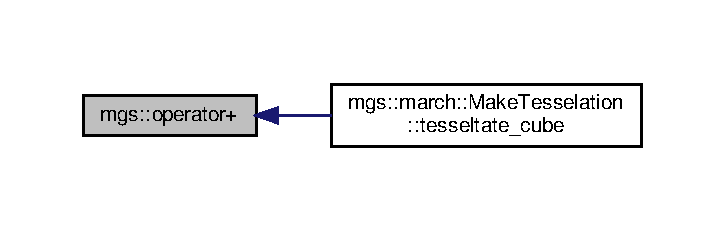
\includegraphics[width=348pt]{namespacemgs_aa3d52c646ace701de74ece1b83e81c3d_icgraph}
\end{center}
\end{figure}
\mbox{\Hypertarget{namespacemgs_aa8de51b8fb971ca949d932b8348298d1}\label{namespacemgs_aa8de51b8fb971ca949d932b8348298d1}} 
\index{mgs@{mgs}!render\+\_\+single\+\_\+cell@{render\+\_\+single\+\_\+cell}}
\index{render\+\_\+single\+\_\+cell@{render\+\_\+single\+\_\+cell}!mgs@{mgs}}
\subsubsection{\texorpdfstring{render\+\_\+single\+\_\+cell()}{render\_single\_cell()}}
{\footnotesize\ttfamily template$<$typename T , typename I $>$ \\
I mgs\+::render\+\_\+single\+\_\+cell (\begin{DoxyParamCaption}\item[{const \hyperlink{structmgs_1_1Vector}{Position} \&}]{initial\+\_\+p,  }\item[{const \hyperlink{structmgs_1_1Vector}{Velocity} \&}]{initial\+\_\+v,  }\item[{const std\+::vector$<$ \hyperlink{structmgs_1_1Star}{Star} $>$ \&}]{stars,  }\item[{const \hyperlink{structmgs_1_1Vector}{Position} \&}]{center\+\_\+of\+\_\+star\+\_\+mass,  }\item[{const \hyperlink{structmgs_1_1FieldParms}{Field\+Parms}$<$ T, I $>$ \&}]{parms,  }\item[{std\+::function$<$ void(const \hyperlink{structmgs_1_1Vector}{Position} \&, const \hyperlink{structmgs_1_1Vector}{Velocity} \&)$>$}]{cb = {\ttfamily nullptr} }\end{DoxyParamCaption})\hspace{0.3cm}{\ttfamily [inline]}}

Iterates a single Free Point Mass from initial position and velocity. This has been pulled out of \hyperlink{structmgs_1_1Field}{Field} to be callable independent of having to set up the entire \hyperlink{structmgs_1_1Field}{Field} object when we are not computing the M\+GS. 
\hypertarget{namespacemgs_1_1march}{}\section{mgs\+:\+:march Namespace Reference}
\label{namespacemgs_1_1march}\index{mgs\+::march@{mgs\+::march}}
\subsection*{Classes}
\begin{DoxyCompactItemize}
\item 
class \hyperlink{classmgs_1_1march_1_1MakeMesh}{Make\+Mesh}
\item 
class \hyperlink{classmgs_1_1march_1_1MakeTesselation}{Make\+Tesselation}
\item 
class \hyperlink{classmgs_1_1march_1_1Pipeline}{Pipeline}
\end{DoxyCompactItemize}
\subsection*{Typedefs}
\begin{DoxyCompactItemize}
\item 
\mbox{\Hypertarget{namespacemgs_1_1march_a0aad9b3e6e0397451a4c792a25c44ca1}\label{namespacemgs_1_1march_a0aad9b3e6e0397451a4c792a25c44ca1}} 
using {\bfseries tetra\+\_\+index\+\_\+t} = std\+::array$<$ \hyperlink{namespacemgs_a40c361242ea98fb1ff1241d06f7d5568}{index\+\_\+bits\+\_\+t}, 4 $>$
\item 
\mbox{\Hypertarget{namespacemgs_1_1march_a81573635f8974f15f4b71b6050e8b38d}\label{namespacemgs_1_1march_a81573635f8974f15f4b71b6050e8b38d}} 
using {\bfseries cube\+\_\+decomposer\+\_\+t} = std\+::array$<$ tetra\+\_\+index\+\_\+t, 6 $>$
\item 
\mbox{\Hypertarget{namespacemgs_1_1march_af86a2a7e7bcb7196097eda7749bf60e0}\label{namespacemgs_1_1march_af86a2a7e7bcb7196097eda7749bf60e0}} 
using {\bfseries pos\+\_\+list\+\_\+t} = std\+::vector$<$ \hyperlink{structmgs_1_1Vector}{Position} $>$
\item 
\mbox{\Hypertarget{namespacemgs_1_1march_ad66d833e33f4513fb34382103bddf074}\label{namespacemgs_1_1march_ad66d833e33f4513fb34382103bddf074}} 
using {\bfseries tetra\+\_\+list\+\_\+t} = std\+::vector$<$ pos\+\_\+list\+\_\+t $>$
\end{DoxyCompactItemize}
\subsection*{Functions}
\begin{DoxyCompactItemize}
\item 
\mbox{\Hypertarget{namespacemgs_1_1march_a34eba5cecd2d1b25d6d0f9b78e9ffc1a}\label{namespacemgs_1_1march_a34eba5cecd2d1b25d6d0f9b78e9ffc1a}} 
std\+::ostream \& {\bfseries operator$<$$<$} (std\+::ostream \&os, pos\+\_\+list\+\_\+t const \&pv)
\item 
\mbox{\Hypertarget{namespacemgs_1_1march_abff648da6f597f80e9d27b67d5e006d6}\label{namespacemgs_1_1march_abff648da6f597f80e9d27b67d5e006d6}} 
std\+::ostream \& {\bfseries operator$<$$<$} (std\+::ostream \&os, \hyperlink{classmgs_1_1march_1_1MakeTesselation}{Make\+Tesselation} const \&tess)
\item 
\mbox{\Hypertarget{namespacemgs_1_1march_aea64facfbf2654abafd500e598eb66e1}\label{namespacemgs_1_1march_aea64facfbf2654abafd500e598eb66e1}} 
std\+::ostream \& {\bfseries operator$<$$<$} (std\+::ostream \&os, tetra\+\_\+list\+\_\+t const \&tl)
\end{DoxyCompactItemize}


\subsection{Detailed Description}
The Marching Tetrahedra is implemented here. We simply wish (for now) to walk the entire field and generate the triangles to render.

T\+O\+DO\+: later on we will optimise this to T\+O\+DO\+: process in a more lazy fashion. For now, T\+O\+DO\+: we will generate a \char`\"{}buffer\char`\"{} of polygons T\+O\+DO\+: that will eventually be rendered. 
\chapter{Class Documentation}
\hypertarget{structmgs_1_1Bounds}{}\section{mgs\+:\+:Bounds Struct Reference}
\label{structmgs_1_1Bounds}\index{mgs\+::\+Bounds@{mgs\+::\+Bounds}}


{\ttfamily \#include $<$compute.\+h$>$}



Collaboration diagram for mgs\+:\+:Bounds\+:
\nopagebreak
\begin{figure}[H]
\begin{center}
\leavevmode
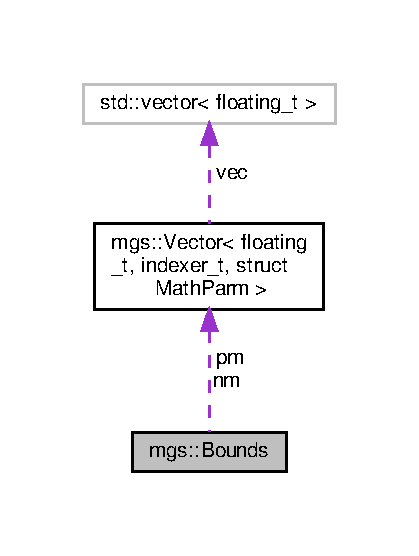
\includegraphics[width=201pt]{structmgs_1_1Bounds__coll__graph}
\end{center}
\end{figure}
\subsection*{Public Attributes}
\begin{DoxyCompactItemize}
\item 
\mbox{\Hypertarget{structmgs_1_1Bounds_a8bfd61fc90b20728aeffdb34c319efa8}\label{structmgs_1_1Bounds_a8bfd61fc90b20728aeffdb34c319efa8}} 
\hyperlink{structmgs_1_1Vector}{Coordinate} {\bfseries nm}
\item 
\mbox{\Hypertarget{structmgs_1_1Bounds_a1c376b96ff5b0193d00e809ee564bcba}\label{structmgs_1_1Bounds_a1c376b96ff5b0193d00e809ee564bcba}} 
\hyperlink{structmgs_1_1Vector}{Coordinate} {\bfseries pm}
\end{DoxyCompactItemize}


\subsection{Detailed Description}
A bounding box for the field 

The documentation for this struct was generated from the following file\+:\begin{DoxyCompactItemize}
\item 
compute/compute.\+h\end{DoxyCompactItemize}

\hypertarget{structmgs_1_1Field}{}\section{mgs\+:\+:Field$<$ T, Iterant, Indexer, P $>$ Struct Template Reference}
\label{structmgs_1_1Field}\index{mgs\+::\+Field$<$ T, Iterant, Indexer, P $>$@{mgs\+::\+Field$<$ T, Iterant, Indexer, P $>$}}


Collaboration diagram for mgs\+:\+:Field$<$ T, Iterant, Indexer, P $>$\+:
\nopagebreak
\begin{figure}[H]
\begin{center}
\leavevmode
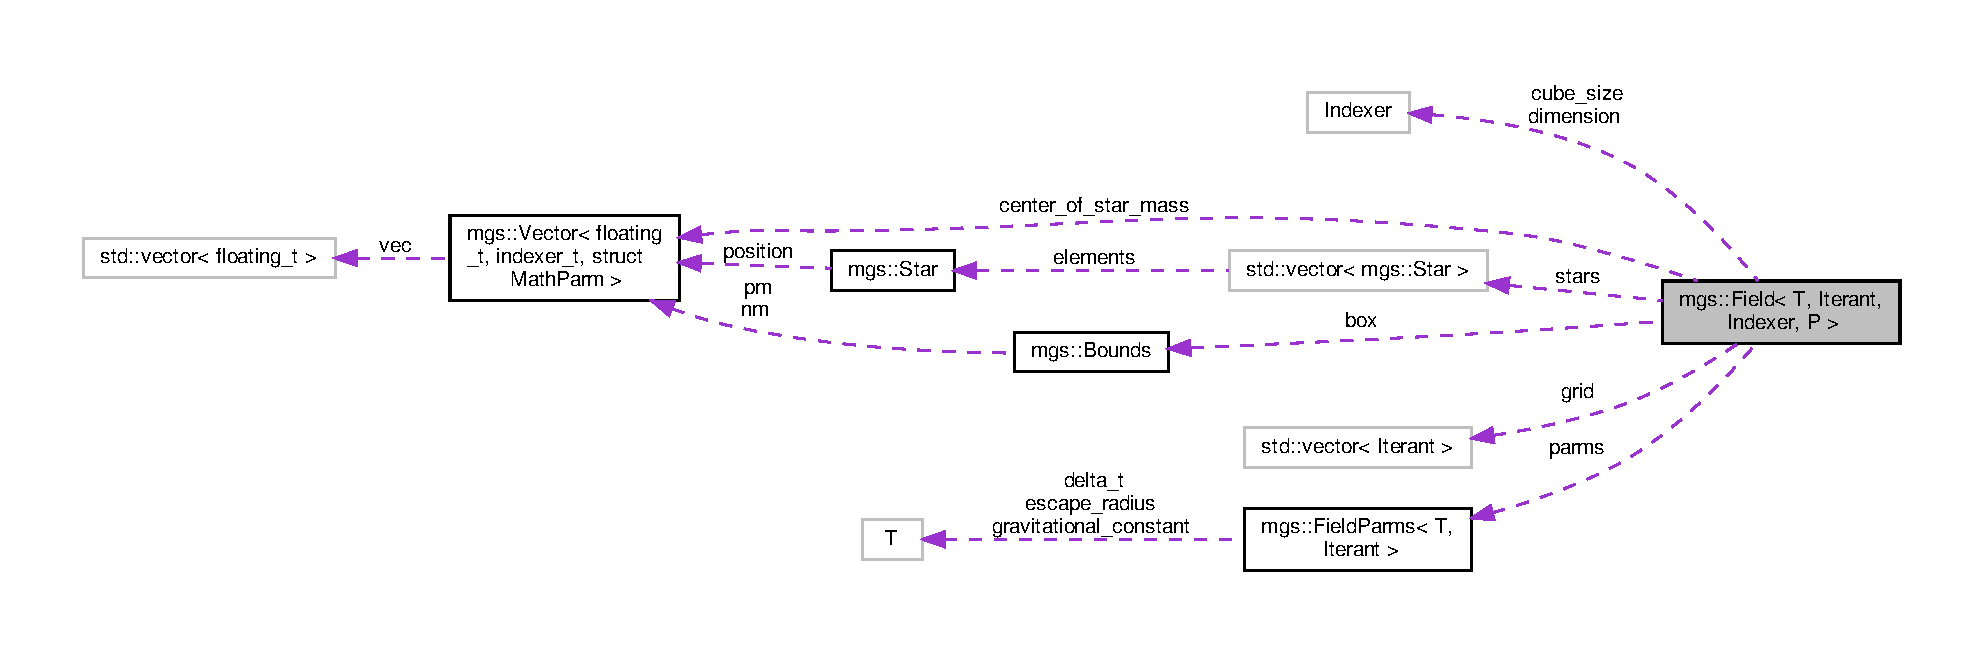
\includegraphics[width=350pt]{structmgs_1_1Field__coll__graph}
\end{center}
\end{figure}
\subsection*{Public Member Functions}
\begin{DoxyCompactItemize}
\item 
\mbox{\Hypertarget{structmgs_1_1Field_a1faa4164faa615f55bb649251b3e344d}\label{structmgs_1_1Field_a1faa4164faa615f55bb649251b3e344d}} 
{\bfseries Field} (\hyperlink{structmgs_1_1Vector}{Coordinate} neg\+\_\+bound, \hyperlink{structmgs_1_1Vector}{Coordinate} pos\+\_\+bound, Iterant cs=256, Iterant dim=2, Iterant iteration\+\_\+limit=1024, T grav\+\_\+constant=1.\+0, T escape\+\_\+r=2.\+0, T delta\+\_\+time=0.\+1)
\item 
\mbox{\Hypertarget{structmgs_1_1Field_ac7a2c770a1f9206aa73f949f4b312f80}\label{structmgs_1_1Field_ac7a2c770a1f9206aa73f949f4b312f80}} 
{\bfseries Field} (\hyperlink{structmgs_1_1Bounds}{Bounds} box\+\_\+, Indexer cs=256, Indexer dim=3, Iterant iteration\+\_\+limit=1024, T grav\+\_\+constant=1.\+0, T escape\+\_\+r=2.\+0, T delta\+\_\+time=0.\+5)
\item 
\mbox{\Hypertarget{structmgs_1_1Field_af82babd1c2f9c0e304698849f1a39ff0}\label{structmgs_1_1Field_af82babd1c2f9c0e304698849f1a39ff0}} 
Iterant \& {\bfseries operator\mbox{[}$\,$\mbox{]}} (const \hyperlink{structmgs_1_1Index}{Index} \&idx)
\item 
\hyperlink{structmgs_1_1Index}{Index} \hyperlink{structmgs_1_1Field_ae10cc38826982adfbf9ef8df7b9bf5bd}{coords2index} (const \hyperlink{structmgs_1_1Vector}{Coordinate} \&c)
\item 
\hyperlink{structmgs_1_1Vector}{Coordinate} \hyperlink{structmgs_1_1Field_a28972ab1f16b45ca949849de53ecf7e7}{index2coordinate} (const \hyperlink{structmgs_1_1Index}{Index} \&idx)
\item 
\mbox{\Hypertarget{structmgs_1_1Field_aa5925b0bbd068b347d69e41cce42ad0e}\label{structmgs_1_1Field_aa5925b0bbd068b347d69e41cce42ad0e}} 
void {\bfseries render\+\_\+with\+\_\+callback} (std\+::function$<$ void(\hyperlink{structmgs_1_1Index}{Index}, \hyperlink{structmgs_1_1Vector}{Position})$>$ cb)
\end{DoxyCompactItemize}
\subsection*{Public Attributes}
\begin{DoxyCompactItemize}
\item 
\mbox{\Hypertarget{structmgs_1_1Field_a3bf519b1216e7019388596b18dc849f5}\label{structmgs_1_1Field_a3bf519b1216e7019388596b18dc849f5}} 
\hyperlink{structmgs_1_1Bounds}{Bounds} {\bfseries box}
\item 
\mbox{\Hypertarget{structmgs_1_1Field_a19d761209af98bb8e3442e0c9dd25892}\label{structmgs_1_1Field_a19d761209af98bb8e3442e0c9dd25892}} 
std\+::vector$<$ Iterant $>$ {\bfseries grid}
\item 
\mbox{\Hypertarget{structmgs_1_1Field_a649eeb6b7f87055cbf6b8d6d60cbcee0}\label{structmgs_1_1Field_a649eeb6b7f87055cbf6b8d6d60cbcee0}} 
std\+::vector$<$ \hyperlink{structmgs_1_1Star}{Star} $>$ {\bfseries stars}
\item 
\mbox{\Hypertarget{structmgs_1_1Field_a9a8507137a87e214e33f256cfebc7ce6}\label{structmgs_1_1Field_a9a8507137a87e214e33f256cfebc7ce6}} 
\hyperlink{structmgs_1_1Vector}{Position} {\bfseries center\+\_\+of\+\_\+star\+\_\+mass}
\item 
\mbox{\Hypertarget{structmgs_1_1Field_a43157fc61030c1eeffe39192fe8a25b2}\label{structmgs_1_1Field_a43157fc61030c1eeffe39192fe8a25b2}} 
Indexer {\bfseries cube\+\_\+size}
\item 
\mbox{\Hypertarget{structmgs_1_1Field_a6d56d193bdc368d461f55a58069cacca}\label{structmgs_1_1Field_a6d56d193bdc368d461f55a58069cacca}} 
Indexer {\bfseries dimension}
\item 
\mbox{\Hypertarget{structmgs_1_1Field_a69de199e9544dd7839ffd5d272fd5982}\label{structmgs_1_1Field_a69de199e9544dd7839ffd5d272fd5982}} 
\hyperlink{structmgs_1_1FieldParms}{Field\+Parms}$<$ T, Iterant $>$ {\bfseries parms}
\end{DoxyCompactItemize}


\subsection{Member Function Documentation}
\mbox{\Hypertarget{structmgs_1_1Field_ae10cc38826982adfbf9ef8df7b9bf5bd}\label{structmgs_1_1Field_ae10cc38826982adfbf9ef8df7b9bf5bd}} 
\index{mgs\+::\+Field@{mgs\+::\+Field}!coords2index@{coords2index}}
\index{coords2index@{coords2index}!mgs\+::\+Field@{mgs\+::\+Field}}
\subsubsection{\texorpdfstring{coords2index()}{coords2index()}}
{\footnotesize\ttfamily template$<$typename T, typename Iterant, typename Indexer, typename P$>$ \\
\hyperlink{structmgs_1_1Index}{Index} \hyperlink{structmgs_1_1Field}{mgs\+::\+Field}$<$ T, Iterant, Indexer, P $>$\+::coords2index (\begin{DoxyParamCaption}\item[{const \hyperlink{structmgs_1_1Vector}{Coordinate} \&}]{c }\end{DoxyParamCaption})\hspace{0.3cm}{\ttfamily [inline]}}

Convert a coordinate Io an index. W\+A\+RN\+: No bounds checking is done here. If a coordinate W\+A\+RN\+: is out of bounds, the index will simply be too high W\+A\+RN\+: or too low (negative), which will result in memory corruption. T\+O\+DO\+: implement some means of bounds checking in \hyperlink{structmgs_1_1Index}{Index} or \hyperlink{structmgs_1_1Field}{Field}. \mbox{\Hypertarget{structmgs_1_1Field_a28972ab1f16b45ca949849de53ecf7e7}\label{structmgs_1_1Field_a28972ab1f16b45ca949849de53ecf7e7}} 
\index{mgs\+::\+Field@{mgs\+::\+Field}!index2coordinate@{index2coordinate}}
\index{index2coordinate@{index2coordinate}!mgs\+::\+Field@{mgs\+::\+Field}}
\subsubsection{\texorpdfstring{index2coordinate()}{index2coordinate()}}
{\footnotesize\ttfamily template$<$typename T, typename Iterant, typename Indexer, typename P$>$ \\
\hyperlink{structmgs_1_1Vector}{Coordinate} \hyperlink{structmgs_1_1Field}{mgs\+::\+Field}$<$ T, Iterant, Indexer, P $>$\+::index2coordinate (\begin{DoxyParamCaption}\item[{const \hyperlink{structmgs_1_1Index}{Index} \&}]{idx }\end{DoxyParamCaption})\hspace{0.3cm}{\ttfamily [inline]}}

Convert an index to coordinate. W\+A\+RN\+: no bounds checking is performed. Here is the caller graph for this function\+:
\nopagebreak
\begin{figure}[H]
\begin{center}
\leavevmode
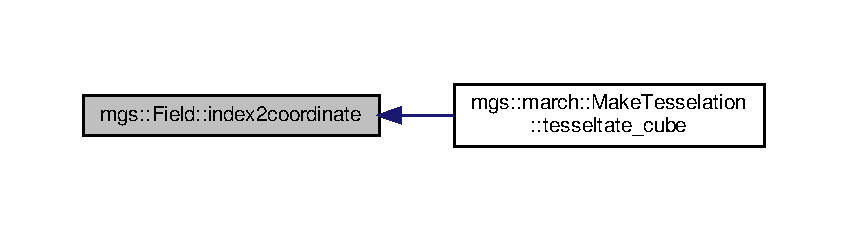
\includegraphics[width=350pt]{structmgs_1_1Field_a28972ab1f16b45ca949849de53ecf7e7_icgraph}
\end{center}
\end{figure}


The documentation for this struct was generated from the following files\+:\begin{DoxyCompactItemize}
\item 
compute/compute.\+h\item 
compute/compute.\+cpp\end{DoxyCompactItemize}

\hypertarget{structmgs_1_1FieldParms}{}\section{mgs\+:\+:Field\+Parms$<$ T, Interant $>$ Struct Template Reference}
\label{structmgs_1_1FieldParms}\index{mgs\+::\+Field\+Parms$<$ T, Interant $>$@{mgs\+::\+Field\+Parms$<$ T, Interant $>$}}


{\ttfamily \#include $<$compute.\+h$>$}



Collaboration diagram for mgs\+:\+:Field\+Parms$<$ T, Interant $>$\+:
\nopagebreak
\begin{figure}[H]
\begin{center}
\leavevmode
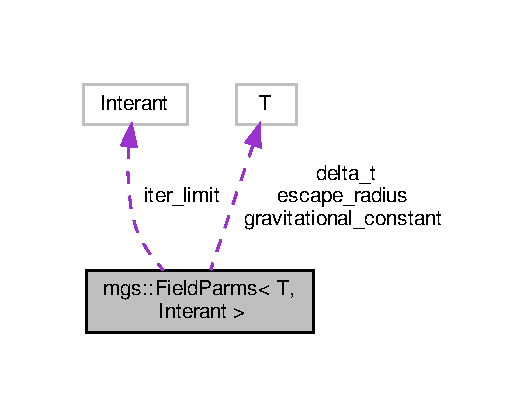
\includegraphics[width=253pt]{structmgs_1_1FieldParms__coll__graph}
\end{center}
\end{figure}
\subsection*{Public Member Functions}
\begin{DoxyCompactItemize}
\item 
\mbox{\Hypertarget{structmgs_1_1FieldParms_adaf0666fe2bbad51d39d46db25a42495}\label{structmgs_1_1FieldParms_adaf0666fe2bbad51d39d46db25a42495}} 
{\bfseries Field\+Parms} (T gc, T dt, Interant il, T er)
\end{DoxyCompactItemize}
\subsection*{Public Attributes}
\begin{DoxyCompactItemize}
\item 
\mbox{\Hypertarget{structmgs_1_1FieldParms_ac087d3d0e4e9d1aa8e9290610327d7f9}\label{structmgs_1_1FieldParms_ac087d3d0e4e9d1aa8e9290610327d7f9}} 
T {\bfseries gravitational\+\_\+constant}
\item 
\mbox{\Hypertarget{structmgs_1_1FieldParms_a46eea5527c0fd40eadcd377dd5b8d97d}\label{structmgs_1_1FieldParms_a46eea5527c0fd40eadcd377dd5b8d97d}} 
T {\bfseries delta\+\_\+t}
\item 
\mbox{\Hypertarget{structmgs_1_1FieldParms_a4ad3c8d11a2f695b89bccbc02d1cb0c5}\label{structmgs_1_1FieldParms_a4ad3c8d11a2f695b89bccbc02d1cb0c5}} 
Interant {\bfseries iter\+\_\+limit}
\item 
\mbox{\Hypertarget{structmgs_1_1FieldParms_ab28959482fd11ba2eb1e37f842d26e8a}\label{structmgs_1_1FieldParms_ab28959482fd11ba2eb1e37f842d26e8a}} 
T {\bfseries escape\+\_\+radius}
\end{DoxyCompactItemize}


\subsection{Detailed Description}
\subsubsection*{template$<$typename T, typename Interant$>$\newline
struct mgs\+::\+Field\+Parms$<$ T, Interant $>$}

\hyperlink{structmgs_1_1Field}{Field} Parameters for M\+GS. These determine the nature of the M\+GS fractal that is generated. 

The documentation for this struct was generated from the following file\+:\begin{DoxyCompactItemize}
\item 
compute/compute.\+h\end{DoxyCompactItemize}

\hypertarget{structmgs_1_1FieldParmsSimulation}{}\section{mgs\+:\+:Field\+Parms\+Simulation$<$ T, I $>$ Struct Template Reference}
\label{structmgs_1_1FieldParmsSimulation}\index{mgs\+::\+Field\+Parms\+Simulation$<$ T, I $>$@{mgs\+::\+Field\+Parms\+Simulation$<$ T, I $>$}}


Inheritance diagram for mgs\+:\+:Field\+Parms\+Simulation$<$ T, I $>$\+:
\nopagebreak
\begin{figure}[H]
\begin{center}
\leavevmode
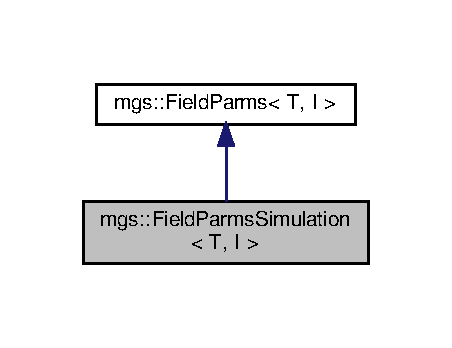
\includegraphics[width=217pt]{structmgs_1_1FieldParmsSimulation__inherit__graph}
\end{center}
\end{figure}


Collaboration diagram for mgs\+:\+:Field\+Parms\+Simulation$<$ T, I $>$\+:
\nopagebreak
\begin{figure}[H]
\begin{center}
\leavevmode
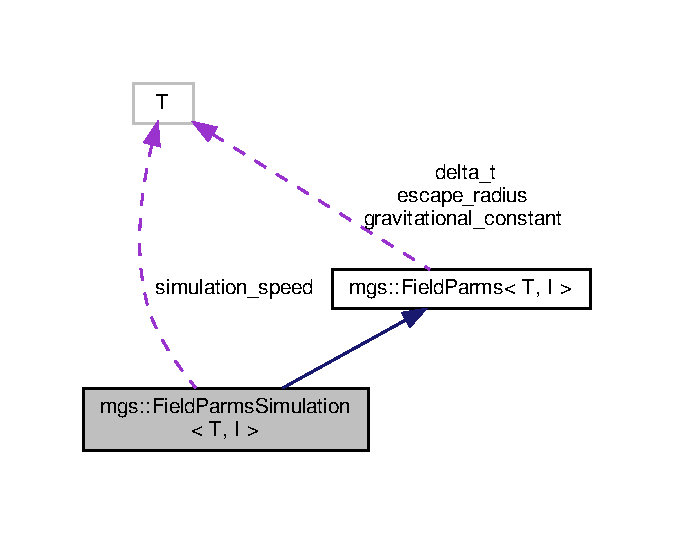
\includegraphics[width=324pt]{structmgs_1_1FieldParmsSimulation__coll__graph}
\end{center}
\end{figure}
\subsection*{Public Member Functions}
\begin{DoxyCompactItemize}
\item 
\mbox{\Hypertarget{structmgs_1_1FieldParmsSimulation_a47d6dbd94d7ade70daf013088942d0eb}\label{structmgs_1_1FieldParmsSimulation_a47d6dbd94d7ade70daf013088942d0eb}} 
{\bfseries Field\+Parms\+Simulation} (T grav\+\_\+const=0.\+01, T dt=0.\+1, I iter=100, T escape\+\_\+r=200, T sim\+\_\+speed=1.\+0)
\end{DoxyCompactItemize}
\subsection*{Public Attributes}
\begin{DoxyCompactItemize}
\item 
\mbox{\Hypertarget{structmgs_1_1FieldParmsSimulation_a947176fc1d7d4b5aaf929616f1bd3a24}\label{structmgs_1_1FieldParmsSimulation_a947176fc1d7d4b5aaf929616f1bd3a24}} 
T {\bfseries simulation\+\_\+speed}
\item 
\mbox{\Hypertarget{structmgs_1_1FieldParms_ac087d3d0e4e9d1aa8e9290610327d7f9}\label{structmgs_1_1FieldParms_ac087d3d0e4e9d1aa8e9290610327d7f9}} 
T {\bfseries gravitational\+\_\+constant}
\item 
\mbox{\Hypertarget{structmgs_1_1FieldParms_a46eea5527c0fd40eadcd377dd5b8d97d}\label{structmgs_1_1FieldParms_a46eea5527c0fd40eadcd377dd5b8d97d}} 
T {\bfseries delta\+\_\+t}
\item 
\mbox{\Hypertarget{structmgs_1_1FieldParms_a4ad3c8d11a2f695b89bccbc02d1cb0c5}\label{structmgs_1_1FieldParms_a4ad3c8d11a2f695b89bccbc02d1cb0c5}} 
I {\bfseries iter\+\_\+limit}
\item 
\mbox{\Hypertarget{structmgs_1_1FieldParms_ab28959482fd11ba2eb1e37f842d26e8a}\label{structmgs_1_1FieldParms_ab28959482fd11ba2eb1e37f842d26e8a}} 
T {\bfseries escape\+\_\+radius}
\end{DoxyCompactItemize}


The documentation for this struct was generated from the following file\+:\begin{DoxyCompactItemize}
\item 
gui/mgs.\+h\end{DoxyCompactItemize}

\hypertarget{structmgs_1_1Index}{}\section{mgs\+:\+:Index Struct Reference}
\label{structmgs_1_1Index}\index{mgs\+::\+Index@{mgs\+::\+Index}}


Collaboration diagram for mgs\+:\+:Index\+:
\nopagebreak
\begin{figure}[H]
\begin{center}
\leavevmode
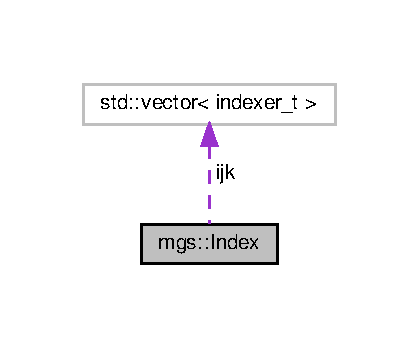
\includegraphics[width=201pt]{structmgs_1_1Index__coll__graph}
\end{center}
\end{figure}
\subsection*{Public Member Functions}
\begin{DoxyCompactItemize}
\item 
\mbox{\Hypertarget{structmgs_1_1Index_a8ef83a7a8f00efc4f25dfff14f0ef92b}\label{structmgs_1_1Index_a8ef83a7a8f00efc4f25dfff14f0ef92b}} 
{\bfseries Index} (std\+::initializer\+\_\+list$<$ indexer\+\_\+t $>$ list)
\item 
\mbox{\Hypertarget{structmgs_1_1Index_a778917404c58bff07205ba5ce03334a5}\label{structmgs_1_1Index_a778917404c58bff07205ba5ce03334a5}} 
{\bfseries Index} (const \hyperlink{structmgs_1_1Index}{Index} \&other)
\item 
\mbox{\Hypertarget{structmgs_1_1Index_a851c30c3cc454ea6e973890e6ae068cc}\label{structmgs_1_1Index_a851c30c3cc454ea6e973890e6ae068cc}} 
{\bfseries Index} (const \hyperlink{structmgs_1_1Index}{Index} \&\&other)
\item 
\mbox{\Hypertarget{structmgs_1_1Index_a6fd3f08fd7b6df7564fdb061e8e2adf8}\label{structmgs_1_1Index_a6fd3f08fd7b6df7564fdb061e8e2adf8}} 
bool {\bfseries operator==} (const \hyperlink{structmgs_1_1Index}{Index} \&other) const
\item 
\mbox{\Hypertarget{structmgs_1_1Index_a983461a967e5e46e5475a2a5097a3ec1}\label{structmgs_1_1Index_a983461a967e5e46e5475a2a5097a3ec1}} 
\hyperlink{structmgs_1_1Index}{Index} \& {\bfseries operator=} (const \hyperlink{structmgs_1_1Index}{Index} \&other)
\item 
\mbox{\Hypertarget{structmgs_1_1Index_adb94c34260974b2c361968fc57746ec5}\label{structmgs_1_1Index_adb94c34260974b2c361968fc57746ec5}} 
\hyperlink{structmgs_1_1Index}{Index} \& {\bfseries operator=} (\hyperlink{structmgs_1_1Index}{Index} \&\&other)
\item 
\mbox{\Hypertarget{structmgs_1_1Index_a7484ae21ad9bb1a3a452948029f138dc}\label{structmgs_1_1Index_a7484ae21ad9bb1a3a452948029f138dc}} 
auto \& {\bfseries operator\mbox{[}$\,$\mbox{]}} (const indexer\+\_\+t \&i)
\item 
\mbox{\Hypertarget{structmgs_1_1Index_a4c2790f9d281294fe162865fe30ab6ac}\label{structmgs_1_1Index_a4c2790f9d281294fe162865fe30ab6ac}} 
auto {\bfseries operator\mbox{[}$\,$\mbox{]}} (const indexer\+\_\+t \&i) const
\item 
\mbox{\Hypertarget{structmgs_1_1Index_a02ef73c597df9571817dc8c5f9020a44}\label{structmgs_1_1Index_a02ef73c597df9571817dc8c5f9020a44}} 
auto {\bfseries size} () const
\end{DoxyCompactItemize}
\subsection*{Public Attributes}
\begin{DoxyCompactItemize}
\item 
\mbox{\Hypertarget{structmgs_1_1Index_a214547444e512d3a56c8dcdd768003dc}\label{structmgs_1_1Index_a214547444e512d3a56c8dcdd768003dc}} 
idx\+\_\+vector\+\_\+t {\bfseries ijk}
\end{DoxyCompactItemize}


The documentation for this struct was generated from the following file\+:\begin{DoxyCompactItemize}
\item 
compute/compute.\+h\end{DoxyCompactItemize}

\hypertarget{classmgs_1_1march_1_1MakeMesh}{}\section{mgs\+:\+:march\+:\+:Make\+Mesh Class Reference}
\label{classmgs_1_1march_1_1MakeMesh}\index{mgs\+::march\+::\+Make\+Mesh@{mgs\+::march\+::\+Make\+Mesh}}


{\ttfamily \#include $<$marching\+\_\+tetrahedra.\+h$>$}



Inheritance diagram for mgs\+:\+:march\+:\+:Make\+Mesh\+:
\nopagebreak
\begin{figure}[H]
\begin{center}
\leavevmode
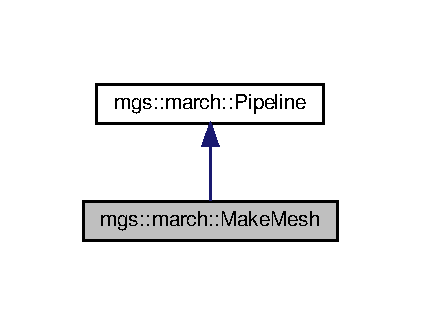
\includegraphics[width=202pt]{classmgs_1_1march_1_1MakeMesh__inherit__graph}
\end{center}
\end{figure}


Collaboration diagram for mgs\+:\+:march\+:\+:Make\+Mesh\+:
\nopagebreak
\begin{figure}[H]
\begin{center}
\leavevmode
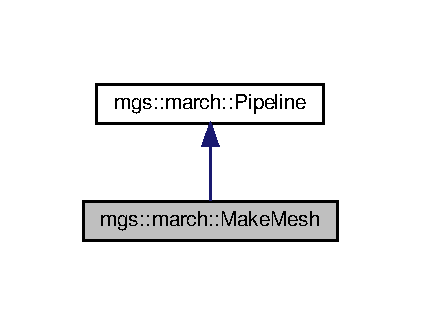
\includegraphics[width=202pt]{classmgs_1_1march_1_1MakeMesh__coll__graph}
\end{center}
\end{figure}
\subsection*{Public Member Functions}
\begin{DoxyCompactItemize}
\item 
\mbox{\Hypertarget{classmgs_1_1march_1_1MakeMesh_a75f2c9780b65330c095ebd8a2d89f148}\label{classmgs_1_1march_1_1MakeMesh_a75f2c9780b65330c095ebd8a2d89f148}} 
{\bfseries Make\+Mesh} (const \hyperlink{classmgs_1_1march_1_1MakeTesselation}{Make\+Tesselation} \&tess)
\end{DoxyCompactItemize}


\subsection{Detailed Description}
We take the results from \hyperlink{classmgs_1_1march_1_1MakeTesselation}{Make\+Tesselation} to now make the mesh. 

The documentation for this class was generated from the following file\+:\begin{DoxyCompactItemize}
\item 
compute/marching\+\_\+tetrahedra.\+h\end{DoxyCompactItemize}

\hypertarget{classmgs_1_1march_1_1MakeTesselation}{}\section{mgs\+:\+:march\+:\+:Make\+Tesselation Class Reference}
\label{classmgs_1_1march_1_1MakeTesselation}\index{mgs\+::march\+::\+Make\+Tesselation@{mgs\+::march\+::\+Make\+Tesselation}}


{\ttfamily \#include $<$marching\+\_\+tetrahedra.\+h$>$}



Inheritance diagram for mgs\+:\+:march\+:\+:Make\+Tesselation\+:
\nopagebreak
\begin{figure}[H]
\begin{center}
\leavevmode
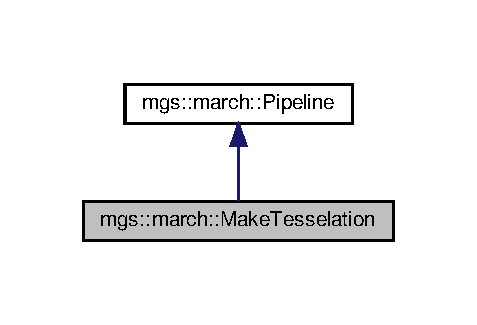
\includegraphics[width=229pt]{classmgs_1_1march_1_1MakeTesselation__inherit__graph}
\end{center}
\end{figure}


Collaboration diagram for mgs\+:\+:march\+:\+:Make\+Tesselation\+:
\nopagebreak
\begin{figure}[H]
\begin{center}
\leavevmode
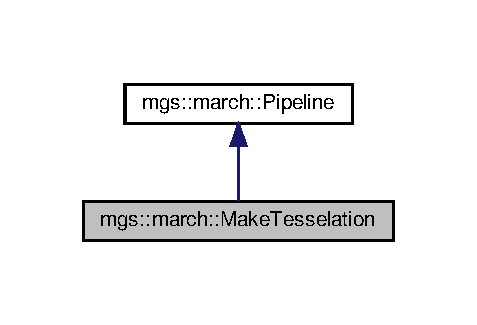
\includegraphics[width=229pt]{classmgs_1_1march_1_1MakeTesselation__coll__graph}
\end{center}
\end{figure}
\subsection*{Public Member Functions}
\begin{DoxyCompactItemize}
\item 
\mbox{\Hypertarget{classmgs_1_1march_1_1MakeTesselation_a20e3550be02146d8560874d3597f1c86}\label{classmgs_1_1march_1_1MakeTesselation_a20e3550be02146d8560874d3597f1c86}} 
{\bfseries Make\+Tesselation} (const \hyperlink{namespacemgs_a7908010cda249b8bf1ea06572a4d4984}{Star\+Field} \&field)
\item 
\mbox{\Hypertarget{classmgs_1_1march_1_1MakeTesselation_a44841d513754e6cee703e6fc006fda14}\label{classmgs_1_1march_1_1MakeTesselation_a44841d513754e6cee703e6fc006fda14}} 
{\bfseries Make\+Tesselation} (const \hyperlink{namespacemgs_a7908010cda249b8bf1ea06572a4d4984}{Star\+Field} \&\&field)
\item 
tetra\+\_\+list\+\_\+t \hyperlink{classmgs_1_1march_1_1MakeTesselation_ace6aa58a0636038e85d187de142e1aa9}{tesseltate\+\_\+cube} (const \hyperlink{structmgs_1_1Index}{Index} \&lmp)
\item 
\mbox{\Hypertarget{classmgs_1_1march_1_1MakeTesselation_a30d8d7305f8d8904f77d9a4f27371430}\label{classmgs_1_1march_1_1MakeTesselation_a30d8d7305f8d8904f77d9a4f27371430}} 
{\footnotesize template$<$typename Shape $>$ }\\Shape {\bfseries operator()} ()
\end{DoxyCompactItemize}
\subsection*{Friends}
\begin{DoxyCompactItemize}
\item 
\mbox{\Hypertarget{classmgs_1_1march_1_1MakeTesselation_aa764f607aa3ba2f179283acdf41c5c7c}\label{classmgs_1_1march_1_1MakeTesselation_aa764f607aa3ba2f179283acdf41c5c7c}} 
std\+::ostream \& {\bfseries operator$<$$<$} (std\+::ostream \&, \hyperlink{classmgs_1_1march_1_1MakeTesselation}{Make\+Tesselation} const \&)
\end{DoxyCompactItemize}


\subsection{Detailed Description}
We create the initial list of polygons here (not necessarily in the form needed for Open\+G\+L!!!) 

\subsection{Member Function Documentation}
\mbox{\Hypertarget{classmgs_1_1march_1_1MakeTesselation_ace6aa58a0636038e85d187de142e1aa9}\label{classmgs_1_1march_1_1MakeTesselation_ace6aa58a0636038e85d187de142e1aa9}} 
\index{mgs\+::march\+::\+Make\+Tesselation@{mgs\+::march\+::\+Make\+Tesselation}!tesseltate\+\_\+cube@{tesseltate\+\_\+cube}}
\index{tesseltate\+\_\+cube@{tesseltate\+\_\+cube}!mgs\+::march\+::\+Make\+Tesselation@{mgs\+::march\+::\+Make\+Tesselation}}
\subsubsection{\texorpdfstring{tesseltate\+\_\+cube()}{tesseltate\_cube()}}
{\footnotesize\ttfamily tetra\+\_\+list\+\_\+t mgs\+::march\+::\+Make\+Tesselation\+::tesseltate\+\_\+cube (\begin{DoxyParamCaption}\item[{const \hyperlink{structmgs_1_1Index}{Index} \&}]{lmp }\end{DoxyParamCaption})}

From the lower most point index, testelate the cube to the upper most point (basically by adding 1 to the indices of the lmp). Here is the call graph for this function\+:
\nopagebreak
\begin{figure}[H]
\begin{center}
\leavevmode
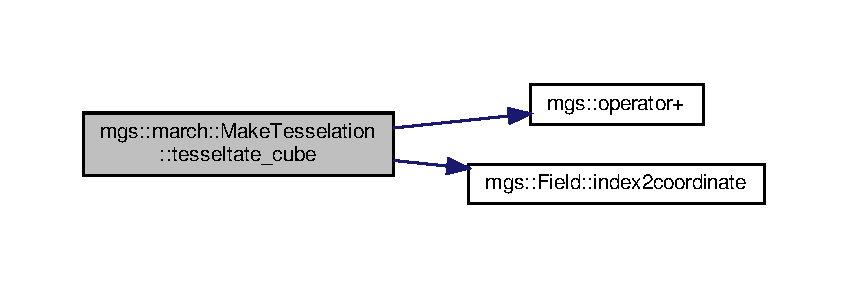
\includegraphics[width=350pt]{classmgs_1_1march_1_1MakeTesselation_ace6aa58a0636038e85d187de142e1aa9_cgraph}
\end{center}
\end{figure}


The documentation for this class was generated from the following files\+:\begin{DoxyCompactItemize}
\item 
compute/marching\+\_\+tetrahedra.\+h\item 
compute/marching\+\_\+tetrahedra.\+cpp\end{DoxyCompactItemize}

\hypertarget{classmgs_1_1march_1_1Pipeline}{}\section{mgs\+:\+:march\+:\+:Pipeline Class Reference}
\label{classmgs_1_1march_1_1Pipeline}\index{mgs\+::march\+::\+Pipeline@{mgs\+::march\+::\+Pipeline}}


{\ttfamily \#include $<$marching\+\_\+tetrahedra.\+h$>$}



Inheritance diagram for mgs\+:\+:march\+:\+:Pipeline\+:
\nopagebreak
\begin{figure}[H]
\begin{center}
\leavevmode
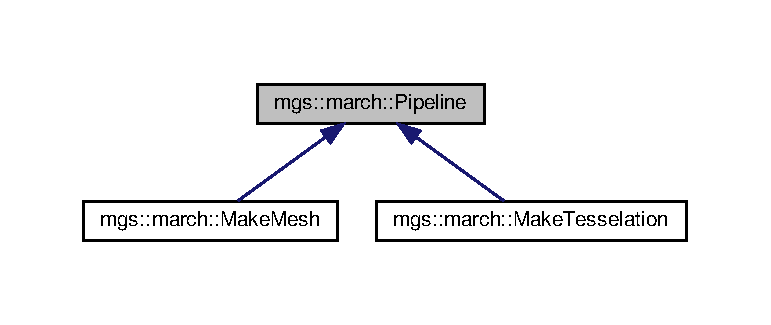
\includegraphics[width=350pt]{classmgs_1_1march_1_1Pipeline__inherit__graph}
\end{center}
\end{figure}


\subsection{Detailed Description}
Production is done in a pipeline fashion, and later will be made lazy. All classes involved in the pipeline shall be derived from this one. 

The documentation for this class was generated from the following file\+:\begin{DoxyCompactItemize}
\item 
compute/marching\+\_\+tetrahedra.\+h\end{DoxyCompactItemize}

\hypertarget{structmgs_1_1PosVel}{}\section{mgs\+:\+:Pos\+Vel Struct Reference}
\label{structmgs_1_1PosVel}\index{mgs\+::\+Pos\+Vel@{mgs\+::\+Pos\+Vel}}


{\ttfamily \#include $<$compute.\+h$>$}



Collaboration diagram for mgs\+:\+:Pos\+Vel\+:
\nopagebreak
\begin{figure}[H]
\begin{center}
\leavevmode
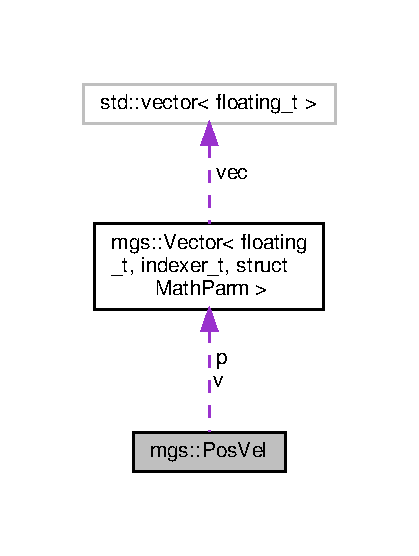
\includegraphics[width=201pt]{structmgs_1_1PosVel__coll__graph}
\end{center}
\end{figure}
\subsection*{Public Attributes}
\begin{DoxyCompactItemize}
\item 
\mbox{\Hypertarget{structmgs_1_1PosVel_aa4b735462e2bb5beae231fabfe600f0c}\label{structmgs_1_1PosVel_aa4b735462e2bb5beae231fabfe600f0c}} 
\hyperlink{structmgs_1_1Vector}{Position} {\bfseries p}
\item 
\mbox{\Hypertarget{structmgs_1_1PosVel_a98404c9fccdf75eed22a077250f60d2e}\label{structmgs_1_1PosVel_a98404c9fccdf75eed22a077250f60d2e}} 
\hyperlink{structmgs_1_1Vector}{Velocity} {\bfseries v}
\end{DoxyCompactItemize}


\subsection{Detailed Description}
For some operations, it helps to have Position and Velocity combined. 

The documentation for this struct was generated from the following file\+:\begin{DoxyCompactItemize}
\item 
compute/compute.\+h\end{DoxyCompactItemize}

\hypertarget{structqt__meta__stringdata__mgs____StarConfig__t}{}\section{qt\+\_\+meta\+\_\+stringdata\+\_\+mgs\+\_\+\+\_\+\+Star\+Config\+\_\+t Struct Reference}
\label{structqt__meta__stringdata__mgs____StarConfig__t}\index{qt\+\_\+meta\+\_\+stringdata\+\_\+mgs\+\_\+\+\_\+\+Star\+Config\+\_\+t@{qt\+\_\+meta\+\_\+stringdata\+\_\+mgs\+\_\+\+\_\+\+Star\+Config\+\_\+t}}
\subsection*{Public Attributes}
\begin{DoxyCompactItemize}
\item 
\mbox{\Hypertarget{structqt__meta__stringdata__mgs____StarConfig__t_ab14aa3cad21319f115b2467a97eaead1}\label{structqt__meta__stringdata__mgs____StarConfig__t_ab14aa3cad21319f115b2467a97eaead1}} 
Q\+Byte\+Array\+Data {\bfseries data} \mbox{[}17\mbox{]}
\item 
\mbox{\Hypertarget{structqt__meta__stringdata__mgs____StarConfig__t_ac5bfa20eb1e0de20368200a4d89c61f2}\label{structqt__meta__stringdata__mgs____StarConfig__t_ac5bfa20eb1e0de20368200a4d89c61f2}} 
char {\bfseries stringdata0} \mbox{[}216\mbox{]}
\end{DoxyCompactItemize}


The documentation for this struct was generated from the following files\+:\begin{DoxyCompactItemize}
\item 
gui/mgs\+\_\+autogen/\+E\+W\+I\+E\+G\+A46\+W\+W/moc\+\_\+star\+\_\+config.\+cpp\item 
gui/mgs\+\_\+autogen/\+E\+W\+I\+E\+G\+A46\+W\+W/moc\+\_\+starconfig.\+cpp\end{DoxyCompactItemize}

\hypertarget{structqt__meta__stringdata__mgs____StarField__t}{}\section{qt\+\_\+meta\+\_\+stringdata\+\_\+mgs\+\_\+\+\_\+\+Star\+Field\+\_\+t Struct Reference}
\label{structqt__meta__stringdata__mgs____StarField__t}\index{qt\+\_\+meta\+\_\+stringdata\+\_\+mgs\+\_\+\+\_\+\+Star\+Field\+\_\+t@{qt\+\_\+meta\+\_\+stringdata\+\_\+mgs\+\_\+\+\_\+\+Star\+Field\+\_\+t}}
\subsection*{Public Attributes}
\begin{DoxyCompactItemize}
\item 
\mbox{\Hypertarget{structqt__meta__stringdata__mgs____StarField__t_ab7649ffd014d55ffcf1a0aa1b5ba7ad3}\label{structqt__meta__stringdata__mgs____StarField__t_ab7649ffd014d55ffcf1a0aa1b5ba7ad3}} 
Q\+Byte\+Array\+Data {\bfseries data} \mbox{[}16\mbox{]}
\item 
\mbox{\Hypertarget{structqt__meta__stringdata__mgs____StarField__t_a51f9ca7794f727ac4a7ee175e5305753}\label{structqt__meta__stringdata__mgs____StarField__t_a51f9ca7794f727ac4a7ee175e5305753}} 
char {\bfseries stringdata0} \mbox{[}222\mbox{]}
\end{DoxyCompactItemize}


The documentation for this struct was generated from the following file\+:\begin{DoxyCompactItemize}
\item 
gui/mgs\+\_\+autogen/\+E\+W\+I\+E\+G\+A46\+W\+W/moc\+\_\+starfield.\+cpp\end{DoxyCompactItemize}

\hypertarget{structqt__meta__stringdata__mgs____StarFieldGUI__t}{}\section{qt\+\_\+meta\+\_\+stringdata\+\_\+mgs\+\_\+\+\_\+\+Star\+Field\+G\+U\+I\+\_\+t Struct Reference}
\label{structqt__meta__stringdata__mgs____StarFieldGUI__t}\index{qt\+\_\+meta\+\_\+stringdata\+\_\+mgs\+\_\+\+\_\+\+Star\+Field\+G\+U\+I\+\_\+t@{qt\+\_\+meta\+\_\+stringdata\+\_\+mgs\+\_\+\+\_\+\+Star\+Field\+G\+U\+I\+\_\+t}}
\subsection*{Public Attributes}
\begin{DoxyCompactItemize}
\item 
\mbox{\Hypertarget{structqt__meta__stringdata__mgs____StarFieldGUI__t_a4e485ef7da8abd87767ea6530322b3c0}\label{structqt__meta__stringdata__mgs____StarFieldGUI__t_a4e485ef7da8abd87767ea6530322b3c0}} 
Q\+Byte\+Array\+Data {\bfseries data} \mbox{[}27\mbox{]}
\item 
\mbox{\Hypertarget{structqt__meta__stringdata__mgs____StarFieldGUI__t_ae808e1c51b536fd13579c94097060dee}\label{structqt__meta__stringdata__mgs____StarFieldGUI__t_ae808e1c51b536fd13579c94097060dee}} 
char {\bfseries stringdata0} \mbox{[}381\mbox{]}
\end{DoxyCompactItemize}


The documentation for this struct was generated from the following file\+:\begin{DoxyCompactItemize}
\item 
gui/mgs\+\_\+autogen/\+E\+W\+I\+E\+G\+A46\+W\+W/moc\+\_\+star\+\_\+field\+\_\+gui.\+cpp\end{DoxyCompactItemize}

\hypertarget{structmgs_1_1SCB}{}\section{mgs\+:\+:S\+CB Struct Reference}
\label{structmgs_1_1SCB}\index{mgs\+::\+S\+CB@{mgs\+::\+S\+CB}}


Collaboration diagram for mgs\+:\+:S\+CB\+:
\nopagebreak
\begin{figure}[H]
\begin{center}
\leavevmode
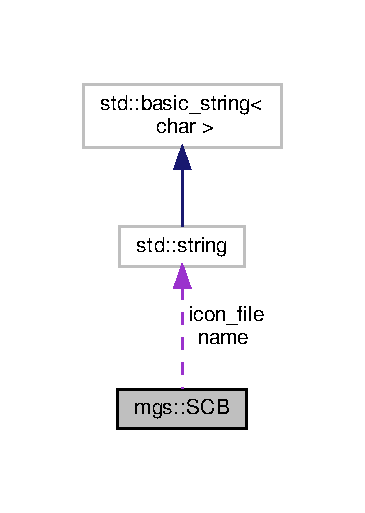
\includegraphics[width=175pt]{structmgs_1_1SCB__coll__graph}
\end{center}
\end{figure}
\subsection*{Public Attributes}
\begin{DoxyCompactItemize}
\item 
\mbox{\Hypertarget{structmgs_1_1SCB_aeb234f5f62710971cec0547ffd399871}\label{structmgs_1_1SCB_aeb234f5f62710971cec0547ffd399871}} 
std\+::string {\bfseries name}
\item 
\mbox{\Hypertarget{structmgs_1_1SCB_a497fb0e8f4dc7433e6552036adc00d22}\label{structmgs_1_1SCB_a497fb0e8f4dc7433e6552036adc00d22}} 
std\+::string {\bfseries icon\+\_\+file}
\item 
\mbox{\Hypertarget{structmgs_1_1SCB_a3efa8f6d825f9178ada2d68a53671ff6}\label{structmgs_1_1SCB_a3efa8f6d825f9178ada2d68a53671ff6}} 
Slot\+G\+UI {\bfseries gslot}
\item 
\mbox{\Hypertarget{structmgs_1_1SCB_a42a2cf2e81cf1a81646b0363feae808f}\label{structmgs_1_1SCB_a42a2cf2e81cf1a81646b0363feae808f}} 
Slot\+CF {\bfseries cslot} = 0
\end{DoxyCompactItemize}


The documentation for this struct was generated from the following file\+:\begin{DoxyCompactItemize}
\item 
gui/star\+\_\+config.\+cpp\end{DoxyCompactItemize}

\hypertarget{structmgs_1_1Star}{}\section{mgs\+:\+:Star Struct Reference}
\label{structmgs_1_1Star}\index{mgs\+::\+Star@{mgs\+::\+Star}}


Collaboration diagram for mgs\+:\+:Star\+:
\nopagebreak
\begin{figure}[H]
\begin{center}
\leavevmode
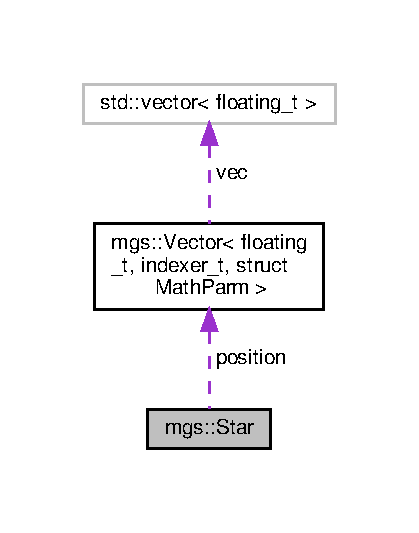
\includegraphics[width=201pt]{structmgs_1_1Star__coll__graph}
\end{center}
\end{figure}
\subsection*{Public Member Functions}
\begin{DoxyCompactItemize}
\item 
\mbox{\Hypertarget{structmgs_1_1Star_a121fa9572ba0a7645a3310beabc25318}\label{structmgs_1_1Star_a121fa9572ba0a7645a3310beabc25318}} 
{\bfseries Star} (floating\+\_\+t m, \hyperlink{structmgs_1_1Vector}{Position} pos)
\end{DoxyCompactItemize}
\subsection*{Public Attributes}
\begin{DoxyCompactItemize}
\item 
\mbox{\Hypertarget{structmgs_1_1Star_a9899c0d2ad809ebaf09fcdbf1754d90e}\label{structmgs_1_1Star_a9899c0d2ad809ebaf09fcdbf1754d90e}} 
floating\+\_\+t {\bfseries mass}
\item 
\mbox{\Hypertarget{structmgs_1_1Star_ac752567d2e017648aa93603f5cfe3b0c}\label{structmgs_1_1Star_ac752567d2e017648aa93603f5cfe3b0c}} 
\hyperlink{structmgs_1_1Vector}{Position} {\bfseries position}
\end{DoxyCompactItemize}


The documentation for this struct was generated from the following file\+:\begin{DoxyCompactItemize}
\item 
compute/compute.\+h\end{DoxyCompactItemize}

\hypertarget{classmgs_1_1StarConfig}{}\section{mgs\+:\+:Star\+Config Class Reference}
\label{classmgs_1_1StarConfig}\index{mgs\+::\+Star\+Config@{mgs\+::\+Star\+Config}}


Inheritance diagram for mgs\+:\+:Star\+Config\+:
\nopagebreak
\begin{figure}[H]
\begin{center}
\leavevmode
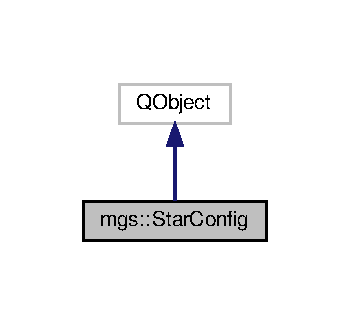
\includegraphics[width=168pt]{classmgs_1_1StarConfig__inherit__graph}
\end{center}
\end{figure}


Collaboration diagram for mgs\+:\+:Star\+Config\+:
\nopagebreak
\begin{figure}[H]
\begin{center}
\leavevmode
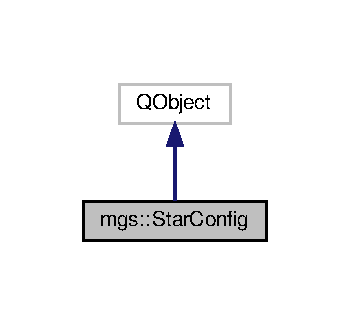
\includegraphics[width=168pt]{classmgs_1_1StarConfig__coll__graph}
\end{center}
\end{figure}
\subsection*{Public Slots}
\begin{DoxyCompactItemize}
\item 
\mbox{\Hypertarget{classmgs_1_1StarConfig_a22e5490b5365f563fe1e7e918b860825}\label{classmgs_1_1StarConfig_a22e5490b5365f563fe1e7e918b860825}} 
void {\bfseries sl\+\_\+select\+\_\+star} (int index, const \hyperlink{structmgs_1_1Star}{Star} \&star)
\item 
\mbox{\Hypertarget{classmgs_1_1StarConfig_ae630911c36a64a5f5ab0791a50473ad7}\label{classmgs_1_1StarConfig_ae630911c36a64a5f5ab0791a50473ad7}} 
void {\bfseries sl\+\_\+set\+\_\+number\+\_\+of\+\_\+stars} (int count)
\item 
\mbox{\Hypertarget{classmgs_1_1StarConfig_a309fb30037cf8a2bbfb301c7fb826594}\label{classmgs_1_1StarConfig_a309fb30037cf8a2bbfb301c7fb826594}} 
void {\bfseries sl\+\_\+star\+\_\+selected} (int index)
\item 
\mbox{\Hypertarget{classmgs_1_1StarConfig_a9c8eea746149f2b8d0a9cedd3c609802}\label{classmgs_1_1StarConfig_a9c8eea746149f2b8d0a9cedd3c609802}} 
void {\bfseries sl\+\_\+star\+\_\+config\+\_\+changed} (const Q\+String \&\+\_\+text)
\item 
\mbox{\Hypertarget{classmgs_1_1StarConfig_a124cf24fbb931a0441374546587eac54}\label{classmgs_1_1StarConfig_a124cf24fbb931a0441374546587eac54}} 
void {\bfseries sl\+\_\+overall\+\_\+config\+\_\+changed} (const Q\+String \&\+\_\+text)
\end{DoxyCompactItemize}
\subsection*{Signals}
\begin{DoxyCompactItemize}
\item 
\mbox{\Hypertarget{classmgs_1_1StarConfig_a695187db1f613d9c86e8acb19e84e342}\label{classmgs_1_1StarConfig_a695187db1f613d9c86e8acb19e84e342}} 
void {\bfseries sig\+\_\+update\+\_\+star} (int index, const \hyperlink{structmgs_1_1Star}{Star} \&star)
\item 
\mbox{\Hypertarget{classmgs_1_1StarConfig_ad16e18ea3ce6269a05726fece52d5207}\label{classmgs_1_1StarConfig_ad16e18ea3ce6269a05726fece52d5207}} 
void {\bfseries sig\+\_\+select\+\_\+star} (int index)
\item 
\mbox{\Hypertarget{classmgs_1_1StarConfig_a11f05400cd60e2383a6630d5b1b8811e}\label{classmgs_1_1StarConfig_a11f05400cd60e2383a6630d5b1b8811e}} 
void {\bfseries sig\+\_\+update\+\_\+overall} (const \hyperlink{structmgs_1_1FieldParmsSimulation}{Overall} \&overall)
\end{DoxyCompactItemize}
\subsection*{Public Member Functions}
\begin{DoxyCompactItemize}
\item 
\mbox{\Hypertarget{classmgs_1_1StarConfig_a07ad69b5260f542bfc5874dc5696365e}\label{classmgs_1_1StarConfig_a07ad69b5260f542bfc5874dc5696365e}} 
void {\bfseries init} ()
\end{DoxyCompactItemize}


The documentation for this class was generated from the following files\+:\begin{DoxyCompactItemize}
\item 
gui/star\+\_\+config.\+h\item 
gui/mgs\+\_\+autogen/\+E\+W\+I\+E\+G\+A46\+W\+W/moc\+\_\+star\+\_\+config.\+cpp\item 
gui/star\+\_\+config.\+cpp\end{DoxyCompactItemize}

\hypertarget{classmgs_1_1StarFieldGUI}{}\section{mgs\+:\+:Star\+Field\+G\+UI Class Reference}
\label{classmgs_1_1StarFieldGUI}\index{mgs\+::\+Star\+Field\+G\+UI@{mgs\+::\+Star\+Field\+G\+UI}}


Inheritance diagram for mgs\+:\+:Star\+Field\+G\+UI\+:
\nopagebreak
\begin{figure}[H]
\begin{center}
\leavevmode
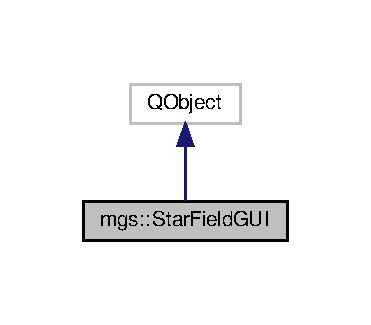
\includegraphics[width=178pt]{classmgs_1_1StarFieldGUI__inherit__graph}
\end{center}
\end{figure}


Collaboration diagram for mgs\+:\+:Star\+Field\+G\+UI\+:
\nopagebreak
\begin{figure}[H]
\begin{center}
\leavevmode
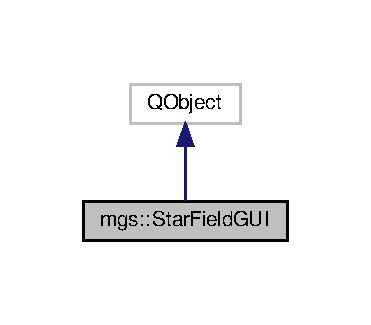
\includegraphics[width=178pt]{classmgs_1_1StarFieldGUI__coll__graph}
\end{center}
\end{figure}
\subsection*{Public Slots}
\begin{DoxyCompactItemize}
\item 
\mbox{\Hypertarget{classmgs_1_1StarFieldGUI_adc5b5b4379524ec391cc70890468a3e8}\label{classmgs_1_1StarFieldGUI_adc5b5b4379524ec391cc70890468a3e8}} 
void {\bfseries sl\+\_\+set\+Free\+Point\+Cube} (int side)
\item 
\mbox{\Hypertarget{classmgs_1_1StarFieldGUI_a8b227afe1170fc81276a6ad39813a1ea}\label{classmgs_1_1StarFieldGUI_a8b227afe1170fc81276a6ad39813a1ea}} 
void {\bfseries sl\+\_\+toggle\+Simulation} ()
\item 
\mbox{\Hypertarget{classmgs_1_1StarFieldGUI_a182881f1c097ea1e4bd7a7b41e07dd5c}\label{classmgs_1_1StarFieldGUI_a182881f1c097ea1e4bd7a7b41e07dd5c}} 
void {\bfseries sl\+\_\+step\+Simulation} ()
\item 
\mbox{\Hypertarget{classmgs_1_1StarFieldGUI_a5323d701751c5ba72ce21b005688b88f}\label{classmgs_1_1StarFieldGUI_a5323d701751c5ba72ce21b005688b88f}} 
void {\bfseries sl\+\_\+toggle\+Center} ()
\item 
\mbox{\Hypertarget{classmgs_1_1StarFieldGUI_a228303f6244f505f0b1a467f7e0de3ec}\label{classmgs_1_1StarFieldGUI_a228303f6244f505f0b1a467f7e0de3ec}} 
void {\bfseries sl\+\_\+toggle\+Arrows} ()
\item 
\mbox{\Hypertarget{classmgs_1_1StarFieldGUI_a56ab30440a65aac07c8a496d2ba18420}\label{classmgs_1_1StarFieldGUI_a56ab30440a65aac07c8a496d2ba18420}} 
void {\bfseries sl\+\_\+make\+\_\+polygon} (int stars)
\item 
\mbox{\Hypertarget{classmgs_1_1StarFieldGUI_ac7bb9f00370166b4c0856ca5446f2f34}\label{classmgs_1_1StarFieldGUI_ac7bb9f00370166b4c0856ca5446f2f34}} 
void {\bfseries sl\+\_\+make\+\_\+tetrahedron} ()
\item 
\mbox{\Hypertarget{classmgs_1_1StarFieldGUI_acaa5c54fb6c8d48ae6dbd2890fef9d59}\label{classmgs_1_1StarFieldGUI_acaa5c54fb6c8d48ae6dbd2890fef9d59}} 
void {\bfseries sl\+\_\+make\+\_\+octahedron} ()
\item 
\mbox{\Hypertarget{classmgs_1_1StarFieldGUI_ad1f2f0f2f8aa154f7b4341478f020063}\label{classmgs_1_1StarFieldGUI_ad1f2f0f2f8aa154f7b4341478f020063}} 
void {\bfseries sl\+\_\+make\+\_\+hexahedron} ()
\item 
\mbox{\Hypertarget{classmgs_1_1StarFieldGUI_a9a64e743e9a5abe5edd74d90247d723e}\label{classmgs_1_1StarFieldGUI_a9a64e743e9a5abe5edd74d90247d723e}} 
void {\bfseries sl\+\_\+make\+\_\+dodecahedron} ()
\item 
\mbox{\Hypertarget{classmgs_1_1StarFieldGUI_a258451580088c6db0382c3e5d52fa732}\label{classmgs_1_1StarFieldGUI_a258451580088c6db0382c3e5d52fa732}} 
void {\bfseries sl\+\_\+make\+\_\+icosahedron} ()
\item 
\mbox{\Hypertarget{classmgs_1_1StarFieldGUI_a439a310ee60d4734dd0f5b113fa63656}\label{classmgs_1_1StarFieldGUI_a439a310ee60d4734dd0f5b113fa63656}} 
void {\bfseries sl\+\_\+star\+\_\+selected} (int index)
\item 
\mbox{\Hypertarget{classmgs_1_1StarFieldGUI_a08ae7d43df6daa06e6db3f134bd5ea13}\label{classmgs_1_1StarFieldGUI_a08ae7d43df6daa06e6db3f134bd5ea13}} 
void {\bfseries sl\+\_\+update\+\_\+star} (int index, const \hyperlink{structmgs_1_1Star}{Star} \&star)
\item 
\mbox{\Hypertarget{classmgs_1_1StarFieldGUI_a99b26bf62f836fcf8c3554e43a66bf6f}\label{classmgs_1_1StarFieldGUI_a99b26bf62f836fcf8c3554e43a66bf6f}} 
void {\bfseries sl\+\_\+reset\+\_\+eularian} ()
\item 
\mbox{\Hypertarget{classmgs_1_1StarFieldGUI_a7134d966b6b9e8e0e7b671e6c56c17a3}\label{classmgs_1_1StarFieldGUI_a7134d966b6b9e8e0e7b671e6c56c17a3}} 
void {\bfseries sl\+\_\+update\+\_\+overall} (const \hyperlink{structmgs_1_1FieldParmsSimulation}{Overall} \&overall)
\item 
\mbox{\Hypertarget{classmgs_1_1StarFieldGUI_a06c48d969b008f9088c25c2c1b442478}\label{classmgs_1_1StarFieldGUI_a06c48d969b008f9088c25c2c1b442478}} 
void {\bfseries sl\+\_\+reset\+\_\+arrows} ()
\end{DoxyCompactItemize}
\subsection*{Signals}
\begin{DoxyCompactItemize}
\item 
\mbox{\Hypertarget{classmgs_1_1StarFieldGUI_af7cc763f4f774ca0d98560ff99a876be}\label{classmgs_1_1StarFieldGUI_af7cc763f4f774ca0d98560ff99a876be}} 
void {\bfseries sig\+\_\+select\+\_\+star} (int index, const \hyperlink{structmgs_1_1Star}{Star} \&star)
\item 
\mbox{\Hypertarget{classmgs_1_1StarFieldGUI_a5b5a5e8023782dff27bccbb170cb0473}\label{classmgs_1_1StarFieldGUI_a5b5a5e8023782dff27bccbb170cb0473}} 
void {\bfseries sig\+\_\+set\+\_\+number\+\_\+of\+\_\+stars} (int count)
\end{DoxyCompactItemize}
\subsection*{Public Member Functions}
\begin{DoxyCompactItemize}
\item 
\mbox{\Hypertarget{classmgs_1_1StarFieldGUI_a2f2a1c01f6de0af4293f1a60e3e4da66}\label{classmgs_1_1StarFieldGUI_a2f2a1c01f6de0af4293f1a60e3e4da66}} 
{\bfseries Star\+Field\+G\+UI} (Q3\+D\+Scatter $\ast$scatter)
\item 
\mbox{\Hypertarget{classmgs_1_1StarFieldGUI_a9867319e53e797a34295c13bf53992b5}\label{classmgs_1_1StarFieldGUI_a9867319e53e797a34295c13bf53992b5}} 
void {\bfseries update\+Field\+State} (bool reset=false)
\item 
\mbox{\Hypertarget{classmgs_1_1StarFieldGUI_a0c971eccc599552e5784cf2e3dba8eb7}\label{classmgs_1_1StarFieldGUI_a0c971eccc599552e5784cf2e3dba8eb7}} 
void {\bfseries clear\+Field} ()
\item 
\mbox{\Hypertarget{classmgs_1_1StarFieldGUI_a2120d8dcc3784be46b516eb2a2586b4d}\label{classmgs_1_1StarFieldGUI_a2120d8dcc3784be46b516eb2a2586b4d}} 
void {\bfseries generate\+Field} ()
\item 
\mbox{\Hypertarget{classmgs_1_1StarFieldGUI_a5a51628c2ef04dc45f7988c5faca9e09}\label{classmgs_1_1StarFieldGUI_a5a51628c2ef04dc45f7988c5faca9e09}} 
void {\bfseries generate\+F\+P\+M\+Initial\+States} ()
\item 
\mbox{\Hypertarget{classmgs_1_1StarFieldGUI_ae1392121b963eeea81b1c77f62787cd9}\label{classmgs_1_1StarFieldGUI_ae1392121b963eeea81b1c77f62787cd9}} 
void {\bfseries eularian\+F\+P\+M\+Advance} ()
\end{DoxyCompactItemize}


The documentation for this class was generated from the following files\+:\begin{DoxyCompactItemize}
\item 
gui/star\+\_\+field\+\_\+gui.\+h\item 
gui/mgs\+\_\+autogen/\+E\+W\+I\+E\+G\+A46\+W\+W/moc\+\_\+star\+\_\+field\+\_\+gui.\+cpp\item 
gui/star\+\_\+field\+\_\+gui.\+cpp\end{DoxyCompactItemize}

\hypertarget{structmgs_1_1Vector}{}\section{mgs\+:\+:Vector$<$ T, Indexer, P $>$ Struct Template Reference}
\label{structmgs_1_1Vector}\index{mgs\+::\+Vector$<$ T, Indexer, P $>$@{mgs\+::\+Vector$<$ T, Indexer, P $>$}}
\subsection*{Public Member Functions}
\begin{DoxyCompactItemize}
\item 
\mbox{\Hypertarget{structmgs_1_1Vector_ac82fe73103a805d2b929271abd06df1b}\label{structmgs_1_1Vector_ac82fe73103a805d2b929271abd06df1b}} 
{\bfseries Vector} (Indexer dimension=default\+\_\+dimension)
\item 
\mbox{\Hypertarget{structmgs_1_1Vector_a6c7ad784dc1039836c852aee99032f9d}\label{structmgs_1_1Vector_a6c7ad784dc1039836c852aee99032f9d}} 
{\bfseries Vector} (std\+::initializer\+\_\+list$<$ T $>$ list)
\item 
\mbox{\Hypertarget{structmgs_1_1Vector_ad3730c7cb5cd6795b221367f862fd40b}\label{structmgs_1_1Vector_ad3730c7cb5cd6795b221367f862fd40b}} 
{\bfseries Vector} (const \hyperlink{structmgs_1_1Vector}{Vector} \&other)
\item 
\mbox{\Hypertarget{structmgs_1_1Vector_adc94ba7d7dae523f54c21c4a1a677597}\label{structmgs_1_1Vector_adc94ba7d7dae523f54c21c4a1a677597}} 
{\bfseries Vector} (const \hyperlink{structmgs_1_1Vector}{Vector} \&\&other)
\item 
\mbox{\Hypertarget{structmgs_1_1Vector_a90ec82d588bf9762cc3869e84dd17acd}\label{structmgs_1_1Vector_a90ec82d588bf9762cc3869e84dd17acd}} 
\hyperlink{structmgs_1_1Vector}{Vector} \& {\bfseries operator=} (const \hyperlink{structmgs_1_1Vector}{Vector} \&other)
\item 
\mbox{\Hypertarget{structmgs_1_1Vector_a865dce16bb24c095efc3aa2362e5e966}\label{structmgs_1_1Vector_a865dce16bb24c095efc3aa2362e5e966}} 
T \& {\bfseries operator\mbox{[}$\,$\mbox{]}} (Indexer index)
\item 
\mbox{\Hypertarget{structmgs_1_1Vector_ad086f4a895249da9ba5490b265df31a6}\label{structmgs_1_1Vector_ad086f4a895249da9ba5490b265df31a6}} 
T {\bfseries operator\mbox{[}$\,$\mbox{]}} (Indexer index) const
\item 
\mbox{\Hypertarget{structmgs_1_1Vector_a4c3d9a6da7f232bde3468129b69925a9}\label{structmgs_1_1Vector_a4c3d9a6da7f232bde3468129b69925a9}} 
auto {\bfseries size} ()
\item 
\mbox{\Hypertarget{structmgs_1_1Vector_a04d59057d40555c84814d60d3d070a95}\label{structmgs_1_1Vector_a04d59057d40555c84814d60d3d070a95}} 
\hyperlink{structmgs_1_1Vector}{Vector} \& {\bfseries operator=} (\hyperlink{structmgs_1_1Vector}{Vector} \&\&other)
\item 
\mbox{\Hypertarget{structmgs_1_1Vector_a0f4f7ad795ba27430b656e792aee1910}\label{structmgs_1_1Vector_a0f4f7ad795ba27430b656e792aee1910}} 
T {\bfseries norm} () const
\item 
\mbox{\Hypertarget{structmgs_1_1Vector_a771d0dadb3f99ace106f67f98e61112b}\label{structmgs_1_1Vector_a771d0dadb3f99ace106f67f98e61112b}} 
T {\bfseries norm\+\_\+squared} () const
\item 
\mbox{\Hypertarget{structmgs_1_1Vector_a41168c8f02222da2fcefec669af1c2ef}\label{structmgs_1_1Vector_a41168c8f02222da2fcefec669af1c2ef}} 
\hyperlink{structmgs_1_1Vector}{Vector} {\bfseries unit\+\_\+vector} () const
\item 
\mbox{\Hypertarget{structmgs_1_1Vector_a48e39771088c8a8a4ccd136d244b7cb2}\label{structmgs_1_1Vector_a48e39771088c8a8a4ccd136d244b7cb2}} 
T {\bfseries dot} (const \hyperlink{structmgs_1_1Vector}{Vector} \&vo) const
\item 
\mbox{\Hypertarget{structmgs_1_1Vector_a0a21795061b9916f01a839df2c77ff5e}\label{structmgs_1_1Vector_a0a21795061b9916f01a839df2c77ff5e}} 
\hyperlink{structmgs_1_1Vector}{Vector} {\bfseries cross} (const \hyperlink{structmgs_1_1Vector}{Vector} \&vo) const
\item 
\mbox{\Hypertarget{structmgs_1_1Vector_a6ffa6e666350344296c61a880ac4cff0}\label{structmgs_1_1Vector_a6ffa6e666350344296c61a880ac4cff0}} 
\hyperlink{structmgs_1_1Vector}{Vector} {\bfseries operator+} (const \hyperlink{structmgs_1_1Vector}{Vector} \&other) const
\item 
\mbox{\Hypertarget{structmgs_1_1Vector_a04ece2322d6b5fabb2782fcfcc837e58}\label{structmgs_1_1Vector_a04ece2322d6b5fabb2782fcfcc837e58}} 
\hyperlink{structmgs_1_1Vector}{Vector} {\bfseries operator+=} (const \hyperlink{structmgs_1_1Vector}{Vector} \&other)
\item 
\mbox{\Hypertarget{structmgs_1_1Vector_a3a5989608b74bb77ceb95b7076d60e17}\label{structmgs_1_1Vector_a3a5989608b74bb77ceb95b7076d60e17}} 
\hyperlink{structmgs_1_1Vector}{Vector} {\bfseries operator-\/} (const \hyperlink{structmgs_1_1Vector}{Vector} \&other) const
\item 
\mbox{\Hypertarget{structmgs_1_1Vector_a7044beae2075e2ea336785a63221d6f6}\label{structmgs_1_1Vector_a7044beae2075e2ea336785a63221d6f6}} 
\hyperlink{structmgs_1_1Vector}{Vector} {\bfseries operator$\ast$} (const floating\+\_\+t scalar) const
\item 
\mbox{\Hypertarget{structmgs_1_1Vector_aa3b290272bce740e9b5b0e16660dced0}\label{structmgs_1_1Vector_aa3b290272bce740e9b5b0e16660dced0}} 
\hyperlink{structmgs_1_1Vector}{Vector} {\bfseries operator/} (const floating\+\_\+t scalar) const
\item 
bool \hyperlink{structmgs_1_1Vector_aabe20a2406bb1f408f47b5d3efc2a9ae}{operator==} (const \hyperlink{structmgs_1_1Vector}{Vector} \&other) const
\end{DoxyCompactItemize}
\subsection*{Public Attributes}
\begin{DoxyCompactItemize}
\item 
\mbox{\Hypertarget{structmgs_1_1Vector_a6ec3364ab67d162ec7c664349839fdf3}\label{structmgs_1_1Vector_a6ec3364ab67d162ec7c664349839fdf3}} 
std\+::vector$<$ T $>$ {\bfseries vec}
\end{DoxyCompactItemize}


\subsection{Member Function Documentation}
\mbox{\Hypertarget{structmgs_1_1Vector_aabe20a2406bb1f408f47b5d3efc2a9ae}\label{structmgs_1_1Vector_aabe20a2406bb1f408f47b5d3efc2a9ae}} 
\index{mgs\+::\+Vector@{mgs\+::\+Vector}!operator==@{operator==}}
\index{operator==@{operator==}!mgs\+::\+Vector@{mgs\+::\+Vector}}
\subsubsection{\texorpdfstring{operator==()}{operator==()}}
{\footnotesize\ttfamily template$<$typename T, typename Indexer, typename P$>$ \\
bool \hyperlink{structmgs_1_1Vector}{mgs\+::\+Vector}$<$ T, Indexer, P $>$\+::operator== (\begin{DoxyParamCaption}\item[{const \hyperlink{structmgs_1_1Vector}{Vector}$<$ T, Indexer, P $>$ \&}]{other }\end{DoxyParamCaption}) const\hspace{0.3cm}{\ttfamily [inline]}}

T\+O\+DO\+: Note that this may not make sense for floats. We\textquotesingle{}ll T\+O\+DO\+: have to add an epsillon here eventually... this is T\+O\+DO\+: mostly for testing. 

The documentation for this struct was generated from the following file\+:\begin{DoxyCompactItemize}
\item 
compute/compute.\+h\end{DoxyCompactItemize}

\hypertarget{classmgs_1_1render_1_1ViewPort}{}\section{mgs\+:\+:render\+:\+:View\+Port Class Reference}
\label{classmgs_1_1render_1_1ViewPort}\index{mgs\+::render\+::\+View\+Port@{mgs\+::render\+::\+View\+Port}}


Inheritance diagram for mgs\+:\+:render\+:\+:View\+Port\+:
\nopagebreak
\begin{figure}[H]
\begin{center}
\leavevmode
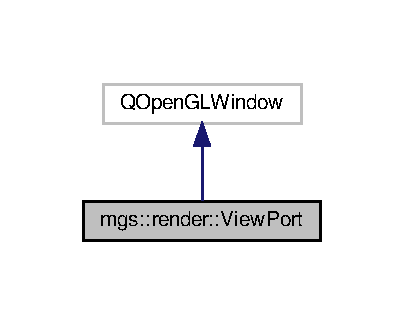
\includegraphics[width=194pt]{classmgs_1_1render_1_1ViewPort__inherit__graph}
\end{center}
\end{figure}


Collaboration diagram for mgs\+:\+:render\+:\+:View\+Port\+:
\nopagebreak
\begin{figure}[H]
\begin{center}
\leavevmode
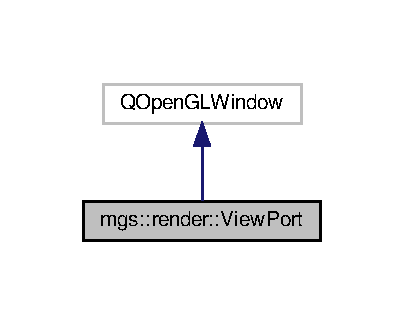
\includegraphics[width=194pt]{classmgs_1_1render_1_1ViewPort__coll__graph}
\end{center}
\end{figure}
\subsection*{Public Slots}
\begin{DoxyCompactItemize}
\item 
\mbox{\Hypertarget{classmgs_1_1render_1_1ViewPort_a477ad01f97f1fb3f4886d00cfbdb8ef6}\label{classmgs_1_1render_1_1ViewPort_a477ad01f97f1fb3f4886d00cfbdb8ef6}} 
void {\bfseries render\+Later} ()
\item 
\mbox{\Hypertarget{classmgs_1_1render_1_1ViewPort_a51212e627debda9cf900227f975bd8d9}\label{classmgs_1_1render_1_1ViewPort_a51212e627debda9cf900227f975bd8d9}} 
void {\bfseries render\+Now} ()
\end{DoxyCompactItemize}
\subsection*{Public Member Functions}
\begin{DoxyCompactItemize}
\item 
\mbox{\Hypertarget{classmgs_1_1render_1_1ViewPort_a2ed0dbb0dbb978a96a0777a41d734d6b}\label{classmgs_1_1render_1_1ViewPort_a2ed0dbb0dbb978a96a0777a41d734d6b}} 
{\bfseries View\+Port} (Q\+Widget $\ast$parent=nullptr)
\item 
\mbox{\Hypertarget{classmgs_1_1render_1_1ViewPort_a0cec33a1673d98d565249a55524f9e16}\label{classmgs_1_1render_1_1ViewPort_a0cec33a1673d98d565249a55524f9e16}} 
void {\bfseries init} (void)
\item 
\mbox{\Hypertarget{classmgs_1_1render_1_1ViewPort_af7f612a71f920c37f93b8f16f6aa556b}\label{classmgs_1_1render_1_1ViewPort_af7f612a71f920c37f93b8f16f6aa556b}} 
virtual void {\bfseries render} (Q\+Painter $\ast$painter)
\item 
\mbox{\Hypertarget{classmgs_1_1render_1_1ViewPort_ab319823d7cc6b6be4281758f4f4801de}\label{classmgs_1_1render_1_1ViewPort_ab319823d7cc6b6be4281758f4f4801de}} 
virtual void {\bfseries render} ()
\item 
\mbox{\Hypertarget{classmgs_1_1render_1_1ViewPort_a4d150f597d41f6911a67076c756de6b6}\label{classmgs_1_1render_1_1ViewPort_a4d150f597d41f6911a67076c756de6b6}} 
virtual void {\bfseries initialize} ()
\item 
\mbox{\Hypertarget{classmgs_1_1render_1_1ViewPort_a27383a1a777d25056f127fd378e17d15}\label{classmgs_1_1render_1_1ViewPort_a27383a1a777d25056f127fd378e17d15}} 
void {\bfseries set\+Animating} (bool animating)
\end{DoxyCompactItemize}
\subsection*{Protected Member Functions}
\begin{DoxyCompactItemize}
\item 
\mbox{\Hypertarget{classmgs_1_1render_1_1ViewPort_af0b0f8d6ddd4a4e3f588e43ecd63400c}\label{classmgs_1_1render_1_1ViewPort_af0b0f8d6ddd4a4e3f588e43ecd63400c}} 
virtual void {\bfseries initialize\+GL} ()
\item 
\mbox{\Hypertarget{classmgs_1_1render_1_1ViewPort_a81be6367e33d0164f36fc5970b9736ee}\label{classmgs_1_1render_1_1ViewPort_a81be6367e33d0164f36fc5970b9736ee}} 
virtual void {\bfseries resize\+GL} (int w, int h)
\item 
\mbox{\Hypertarget{classmgs_1_1render_1_1ViewPort_a926fdab4fa698afc29f1e37a9633510f}\label{classmgs_1_1render_1_1ViewPort_a926fdab4fa698afc29f1e37a9633510f}} 
virtual void {\bfseries paint\+GL} ()
\item 
\mbox{\Hypertarget{classmgs_1_1render_1_1ViewPort_a9a2f33944eb2de7f823bbdb3d6cfc56b}\label{classmgs_1_1render_1_1ViewPort_a9a2f33944eb2de7f823bbdb3d6cfc56b}} 
void {\bfseries paint\+Event} (Q\+Paint\+Event $\ast$event) override
\item 
\mbox{\Hypertarget{classmgs_1_1render_1_1ViewPort_afc88527a95f46869316703c004293fe2}\label{classmgs_1_1render_1_1ViewPort_afc88527a95f46869316703c004293fe2}} 
bool {\bfseries event} (Q\+Event $\ast$event) override
\end{DoxyCompactItemize}


The documentation for this class was generated from the following files\+:\begin{DoxyCompactItemize}
\item 
gui/viewport.\+h\item 
gui/viewport.\+cpp\end{DoxyCompactItemize}

%--- End generated contents ---

% Index
\backmatter
\newpage
\phantomsection
\clearemptydoublepage
\addcontentsline{toc}{chapter}{Index}
\printindex

\end{document}
